%!TEX root = ../thesis.tex

\newcommand{\todo}[1]{\textit{\textcolor{violet}{{#1}}}}

\chapter{Background} 
\label{chapter:intro}

\ifpdf
    \graphicspath{{Introduction/Figs/Raster/}{Introduction/Figs/PDF/}{Introduction/Figs/}}
\else
    \graphicspath{{Introduction/Figs/Vector/}{Introduction/Figs/}}
\fi

%\nomenclature[a-massx]{$M_\oplus$}{mass of Earth [kg]} 
%\nomenclature[a-radiusx]{$R_\oplus$}{radius of Earth [km]}  
\nomenclature[s-aaaaearth]{$\oplus$}{value for Earth}  
\nomenclature[a-temp]{$T$}{temperature [K]}
\nomenclature[a-pressure]{$P$}{pressure [Pa]}
\nomenclature[a-fzo]{$f_{{\rm O}_2}$}{oxygen fugacity}
\nomenclature[z-iw]{IW}{iron-w\"ustite mineral redox buffer}
\nomenclature[z-fmq]{FMQ}{fayalite-magnetite-quartz mineral redox buffer}
\nomenclature[a-log]{log}{always the base-10 logarithm}


%Welcome to my thesis. Nothing to see here---turn the page for science.




The interior of a terrestrial planet shapes its outer character. The surface \textit{-spheres}\footnote{The atmosphere, hydrosphere, cryosphere, biosphere...} known to Earth system scientists owe their existence to motions in the mantle and core. An easy illustration comes with the Moon, which is ``dead", geodynamically, and bare, surficially---it certainly has no atmosphere or hydrosphere, in this case because it is too small and cold to maintain either. The processes that transport energy and matter \textit{through} rocky planets are continuously modulating the qualities of surfaces that emerge from them. These processes determine, to formulaically name some examples, %the core-to-mantle ratio or so-called ``interior structure" \citep[metal core differentiation and redox chemistry; e.g.,][]{li_geochemistry_1996, wade_core_2005, Wood2006, schaefer_metal-silicate_2017, lichtenberg_redox_2021}, 
the lithology of the early crust \citep[the productivity and composition of mantle melting; e.g.,][]{mckenzie_volume_1988, fraeman_influence_2010, HERZBERG2010, wade_divergent_2017, tosi_mercury_2019, dyck_effect_2021, reynard_primordial_2022}, the global tectonic regime \citep[the mysteries of subduction initiation; e.g.,][]{valencia_inevitability_2007, valencia_convection_2009, korenaga_likelihood_2010, foley_conditions_2012, orourke_terrestrial_2012, noack2014can, noack_plate_2014}, the persistence of a shielding magnetic field \citep[outer core convection inducing a geodynamo; e.g.,][]{sharpe_thermal_1978, nimmo_why_2002, gaidos_thermodynamic_2010, boujibar_superearth_2020, zhang_thermal_2022}, and the scope for volcanic greenhouse gas build-up \citep[feasibility of and redox conditions during magmatism; e.g.,][]{kite2009geodynamics, noack_coupling_2012, vilella_fully_2017, ortenzi_mantle_2020, krissansen-totton_was_2021, honing_early_2021, baumeister_redox_2023}. We expect these and numerous other processes to vary, deterministically and stochastically, across the many billions of small planets in our galaxy \citep{cassan_one_2012}, which will, through often-complex, chaotic, interlocking pathways, ultimately manifest as diversity in surface conditions and in the corresponding parameter space of prebiotic environments \citep{walton_can_2022}.


Understanding the cosmic breadth of rocky worlds therefore hinges on understanding their interiors. Yet this reasoning has, for practical reasons, not always directed the planetary astronomer's literature. Telescope observers would struggle to see inside these distant rocks, hence the focus on their atmospheres.\footnote{Telescope imaging cannot directly spatially resolve small planets' surfaces either, due to the fundamentally diffraction-limited angular resolution of optical systems.\label{foot:diffraction-limit}} Nonetheless, the study of planets and moons has historically belonged to astronomy, given the monumental work in that field needed to merely observe these objects' existence in the first place. From modern astronomy's very inception, observers could not help but speculate on how what they saw expanded their conceptions of Earth as a geological entity,\footnote{``Now, is it not the case on the Earth before sunrise, that while the level plain is still in shadow, the peaks of the most lofty mountains are illuminated by the Sun's rays? \ldots The grandeur, however, of such prominences and depressions in the Moon seems to surpass both in magnitude and extent the ruggedness of the Earth's surface, as I shall hereafter show \ldots '' {\sc Galileo Galilei, \textit{The Sidereal Messenger}, 1610 (trans. Edward Stafford Carlos).} Galileo reveals himself as a proto-comparative planetologist with this analysis of lunar topography.} 
%\footnote{``If any one wishes to revive the old opinion of the Pythagoreans, that the Moon is another Earth, so to say, the brighter portion [of the Moon] may very fitly represent the surface of the land, and the darker the expanse of water. Indeed, I have never doubted that if the sphere of the Earth were seen from a distance, when flooded with the Sun's rays, that part of the surface which is land would present itself to view as brighter, and that which is water as darker in comparison.' ' Galileo Galilei, \textit{The Sidereal Messenger}, 1610 (trans. Edward Stafford Carlos).}
 and it is arguable that the question of whether exoplanets exist ``like Earth'' (here usually meaning temperate, wet-but-not-too-wet, maybe inhabited) around other stars is, either implicitly or explicitly, the overarching guideline of contemporary exoplanet astronomy \citep[e.g.,][]{decadalsurveyonastronomyandastrophysics2020astro2020_pathways_2021}. Detailed inquiry into the nature of Earth (``geoscience'' in today's terms) has therefore always been part of the exoplanet project: planets are not stars \citep{taylor_why_2004}.
%\bigskip
%\medskip


% possibly separate this paragraph into one about general modelling philosophy and one outlining thermal history model? probably fine as long as you segue next bit better so it blends in and is not just a. model 1 b. model 2
So long as the surfaces of small planets are probably not, with any reliability, directly detectable for the near future \citep[see also footnote \ref{foot:diffraction-limit}]{teinturier_mapping_2022}, major questions about why---and what fraction of---these planets may or may not develop self-regulating climates, continents with their geochemical niches, surface water, \textit{etc.}, must be attacked first from the theoretical side. That is, we need models which go beyond ``variations on a theme of Earth'' \citep{unterborn_exogeoscience_2020} to probe the potential diversity of planets which are not yet detected. %, in terms of aspects which may never be detectable
The task of physically modelling a planet from scratch may seem ridiculous and impossible. Yet with limitations attended to and uncertainties acknowledged \citep[e.g.,][]{seales_assessing_2019}, the right question/method combination can yield enormously informative results. It is important for the reader to recognise that the worthwhile modelling efforts in this field are often querying the broad senses of change, %(of some unobservable attribute with an observeable input parameter, e.g.)
more so than aiming for small-picture precision. Two classes of planetary interior models form the backbone of this thesis. Both were developed to study the planet Earth, but the methods can be generalised to any planet in principle.

\paragraph{Thermal history models} 

For those interested in a planet's dynamic evolution, modelling the underlying energy balance of the mantle is ubiquitous practice. Accordingly called ``thermal history" models, these calculate large-scale changes in the thermal state of the planet-system over time. Indeed, silicate mantles are both the most massive and the most sluggish ``box'' in such systems \citep{bercovici_mantle_2011}. Thermal history experiments pepper the exoplanet literature with various bespoke complexities layered on, depending on the research question at hand: magmatism, for example, or the transport of water, or the solidification of the liquid-Fe outer core. Yet choosing the proper complexities is an art in itself, as each part of a real planet clearly cannot be coupled to the last detail. Many planetary processes are also still not understood well enough to incorporate into deterministic models directly, or they are nondeterministically path-dependent \citep[no model is expected to predict the tectonic mode of a mature exoplanet \textit{a priori}, e.g.;][]{lenardic_notion_2012, lenardic_solar_2016, weller_evolution_2018}. %Nevertheless, planet evolution models certainly do not have to be complex to be useful. The maximum level of complexity needed for a given problem is that it suffices to remember that the very simplest and earliest thermal history models have probably shown some important stuff about Earth's evolution.} 
Thermal history models are introduced in more detail in section \ref{sec:background-thermalhistory}; Chapters \ref{chapter:topography} and \ref{chapter:outgassing} will rely on them heavily, embodying their multifarious complexity of implementation.%\todo{, which address \textit{how} two different dynamic processes operate on early Earth and exoplanets}.


\paragraph{Phase equilibria models}

% this paragraph brings up something we can do with real astronomical observations - thermal history is maybe stuck in that most of the current work is on arguing about its limitations? (seales and lenardic would disagree tho) an example of a new (~5 yrs) and innovative use of things developed for earth that fit very well into astronomical stuff. lots of exciting new things to do in the near future.  
Another key modelling tool from the planet theory repertoire has origins in petrology. Algorithms to compute petrologic phase diagrams, showing which mineral (and fluid) phases in a system are stable with temperature and pressure, were developed for broad application to Earth's igneous and metamorphic systems \citep[e.g.,][]{thompson_reaction_1982, connolly_algorithm_1987, connolly_geodynamic_2009, asimow_algorithmic_1998, ghiorso_pmelts_2002, stixrude_thermodynamics_2011}. More recently, resourceful exoplaneteers \citep[e.g.,][]{dorn_can_2015, dorn_bayesian_2017, dorn_generalized_2017, dorn_new_2019, unterborn_effects_2017, hinkel_star_2018, putirka_composition_2019, wang_enhanced_2019, wang_detailed_2022, otegi_impact_2020, spaargaren_influence_2020, spaargaren_plausible_2022} have started applying the same models to probe phase proportions in exoplanets. The derived constraints on exoplanet mantle mineralogy, and their cascade of implications, are only just entering the discourse (section \ref{sec:background-composition}). Chapters \ref{chapter:rockywater} and \ref{chapter:fo2} detail my own explorations into phase equilibria modelling. %\todo{This has opened a big door for understanding relatively concrete aspects of planet diversity given that what the thing is made of is such a low order factor, also a good basis for directing experimental petrology.} 


\fancybreak

% what observations tell us about Earth

I have asserted why Earth science illuminates exoplanets. The converse is true as well. Understanding exoplanets is good for Earth science---if nothing else, exoplanets are large-number statistics. Exoplanet data-breadth complements Earth data-depth, such that we might ultimately compare planet evolution outcomes in a passive cosmic clinical trial \citep{shorttle_why_2021, lenardic_habitability_2021}. %The middling first few confirmed exoplanet detections already revealed planetary systems unlike the one we know, demographically-speaking \todo{[REFS]}.
An interesting example of using exoplanet statistics to test a prominent Earth science concept is to look for a pattern between incident stellar luminosity and atmospheric \ce{CO2} abundance \citep{bean_statistical_2017, checlair_statistical_2019, lehmer_carbonatesilicate_2020}---it may tell us that a carbonate-silicate weathering feedback \citep{walker_negative_1981} really does buffer planet surface temperatures \citep[see][]{graham_thermodynamic_2020, penman_silicate_2020}.


Astronomy statistics have already re-framed Earth. With thousands of catalogue rows and counting, rigorous effort has been spent obtaining the underlying occurrence rate of planets, as a function of their radius\footnote{Radius, more often than mass, because so many of these planets were found by transit (i.e., photometric stellar occultation), which measures this. Only a small subset of confirmed planets have both their radius and mass measured thus far.} \citep[e.g.,][]{foreman-mackey_exoplanet_2014, rogers_most_2015, herman_revisiting_2019, bryson_probabilistic_2020, kunimoto_searching_2020, kunimoto_combining_2021, bryson_occurrence_2021, jin_relative_2021}. Among other things, the first statistical exoplanet revolution showed not only that \textit{(i)} smaller planets are more common than giant ones, despite being harder to find (promising if we are looking for empirical Earth ``match pairs''); but more strangely, \textit{(ii)}, %roughly one in five spectrally Sun-like stars have a 
there is a significant population of planets with mysteriously intermediate radius between Earth's and roughly double it. This second point in particular prompted a synchronous foray into how mantle dynamics behave at higher planet mass \citep[e.g.,][]{kite2009geodynamics, valencia_convection_2009, gaidos_thermodynamic_2010, karato_rheological_2011, foley_conditions_2012, stamenkovic_influence_2012, kameyama_stability_2013, tackley_mantle_2013}. Obvious questions of planet (size) diversity still hang: are we just finding big terrestrial planets---or something categorically different? Do they have land surfaces, topography, warm little ponds \citep{darwin_ponds}?
%\footnote{``But if (and oh what a big if) we could conceive in some warm little pond with all sorts of ammonia and phosphoric salts,—light, heat, electricity \& c. present, that a protein compound was chemically formed, ready to undergo still more complex changes...'' \textsc{Charles Darwin}, }?

Stepping back, however, the observational data\footnote{One can infer these low-order compositional classifications---e.g., rocky, icy, gaseous---by comparing precise measurements of a planet's bulk density (from mass and radius) to theoretical mass-radius relationships of different reference compositions, which are calculated from equations of state \citep[in practice, more sophisticated chemical constraints can be leveraged via Markov chain Monte Carlo methods; cf.][]{dorn_bayesian_2017}. However, the meeting of at least three compositional layer possibilities with two measured constraints make this problem fundamentally degenerate, as I discuss in section \ref{sec:background-composition}.} do not support all, or even most, of the known, roughly-Earth-sized planets having Earth-like (or Venus-like, or Mars-like) compositions  \citep{luque_density_2022, rogers_conclusive_2023}. Rather, some intermediate planets have disproportionately small measured masses, implying bulk densities that would make them lighter than a pure compressible sphere of \ce{MgSiO3} \citep[e.g.,][section \ref{sec:background-redox}]{dorn_bayesian_2017, dorn_assessing_2018, schulze_probability_2020}. Therefore, even if they somehow never formed a metal core \citep[see][]{elkins-tanton_coreless_2008}, these planets would still require a low-density component, such as a water layer, of sufficient proportion to match the density constraint. % (The presence of a dense metal core would require even more of this low-density component for the same constraint.) 
Ongoing analysis remains inconclusive about the nature of these light layers, how they are acquired or lost, whether the rocky and volatile-rich populations are linked, and whether this explains the observed distribution of small planet radii \citep[and references therein]{neil_evaluating_2022, rogers_conclusive_2023}. The point being that exoplanet observations continue to surprise us. Our theories are constantly revised, in other words. It is not clear whether our pursuit of this theory has an endgame: if there are universal principles that can explain why all, or most, rocky planets evolve as they do. Relatedly, as I refer to a ``prototypical" planet, I am not pointing to a real object. 
%So whilst I will talk about general trends throughout this thesis, 
It is important to remember that most of the planets in this thesis are abstrations controlled by me.

%silly abstractions controlled by me, not things in the sky.  %\todo{all the planets in this thesis are fake!} 



%Determining an exoplanet's low-order, interior layered structure is notoriously degenerate because mass and radius (bulk density) measurements provide two constraints, but in most cases there are at least three unknowns: the core mass fraction, the rocky mantle mass fraction, and also the possible contribution of a thick gaseous or icy enveloper.











%\todo{Advances brought on by the characterisation era of exoplanet science (i.e., atmospheric spectroscopy) do actually enable some level of statistical inference about planets' interiors, through refined measurements of their radii, masses, and host star chemistry. The lowest-order composition parameter of a planet is its core mass fraction, but small planets could also have a thick layer of gas or ice}
% interior characterisation through measurements of a planet's bulk density, the host star chemistry, and the detection of atmospheric species \citep{santos_constraining_2017, dorn_generalized_2017, dorn_bayesian_2017, dorn_interior_2018, bower_linking_2019, madhusudhan_interior_2020, adibekyan_compositional_2021, wilson_characterising_2022}. 



%In the interim, before more detailed observational constraints on massive potentially-rocky planets can be made, there grows a theoretical literature on how geophysical matters scale with mass: internal structure \citep{valencia_internal_2006, zeng_simple_2017}, tidal response \citep{tobie_tidal_2019}, outgassing \citep{kite_geodynamics_2009, noack_volcanism_2017,dorn_outgassing_2018}, geodynamos \citep{gaidos_thermodynamic_2010}, tectonics \citep{oneill_geological_2007, korenaga_likelihood_2010}, and so on. Here we are interested in the planet mass-scaling of a particular expression of interior dynamics not typically considered in the exoplanet context: the occurence of topography. Topography is tightly linked to temperatures and mantle flows inside the planet. Therefore the problem is one of understanding a planet's thermal history.




\section{Terrestrial planet interiors through time}
\label{sec:background-thermalhistory}
\nomenclature[a-ur]{Ur}{Urey ratio}  
\nomenclature[a-nu]{Nu}{Nusselt number}  
\nomenclature[a-radiusp]{$R_p$}{planet radius [m]}  

% peter: unsolved problems in the field - what are the limits of convection models, what aspects can we justify and what aspects can we not predict?
% because we don't fully understand certain influences on convection, we will be limited in being able to predict ...

%The aims of this section are to introduce mantle thermal evolution via convection as a ``central theory for how the Earth\footnote{and rocky planets by extension!} works'' \citep{bercovici_mantle_2011}, and to discuss how meaningful convection models can be in the context of comparative planetary evolution. 

Planets are born hot with the energy of accretion, produce more heat internally as radioisotopes decay, and over time lose this heat to space \citep{schubert_whole_1980, davies_thermal_1980, moore_heatpipe_2017, lourenco_efficient_2018}. Heat moves through a planet's mantle by convection; mantle convection is what governs the energy available to drive the geologic movements within a planet which fundamentally alter its surface \citep{breuer_dynamics_2015}. Models of mantle convection are therefore the foremost tool we have to predict the variation in these energy flows for different rocky planets, and the different energy-driven evolutions that result: from volcanism and volatile cycling to topography. 

This approach is obviously limited. We have tried for many decades to extrapolate convection models backwards in time from Earth's present-day state, and we have not agreed upon a thermal history that meets all geophysical and geochemical constraints \citep[and references therein]{korenaga_urey_2008}. It is therefore reasonable to ask why we should use these models to predict anything about distant exoplanets. However, those working on Earths' thermal history have also inadvertently started with the hardest problem. Earth is bizarre, geodynamically-speaking, because its surface has developed tectonic plates---at least among the extremely small sample of terrestrial planets whose surface tectonic mobility is to some degree observeable \citep{stern_stagnant_2018}---how these plates interact with the convecting mantle below is complicated and largely unsolved \citep[see][]{lenardic_internal_2022}. Meanwhile,  models of a simpler prototype, a ``stagnant lid'' planet with a thick immobile lithosphere %, can at least consistently explain scaled-down analogues of mantle convection in the laboratory 
(\citealt{davaille_transient_1993, moresi_numerical_1995}; see section \ref{sec:intro-tectonicmode}), have been applied to other solar system bodies with good agreement between models, rooted in the empirically- and numerically-established physics of fluid dynamics \citep[e.g.,][]{plesa_thermal_2015, thiriet_scaling_2019}. Using stagnant lid convection models, we can investigate the thermal evolution of hypothetical exoplanets as we vary, for example, planet size. These kinds of computational experiments can identify large-scale trends \textit{within defined, prototypical convection regimes}---this is currently the depth of analysis we can reach with exoplanets. The converse is that one should be cautious extrapolating models tuned to, for example, Earth's current surface heat flux \citep[e.g.,][]{schubert_whole_1980}, probably a specific feature of its unique geodynamic history.
% here could also mention that specific models developed for rectangular convection or bottom-only won't necessarily extrapolate to differeng geometries and heating modes.


When investigating the thermal evolution of planets in more detail, we may find ourselves blocked by our own currently-limited understanding of certain complex phenomena related to mantle convection. Attempts at incoporating these phenomena into 1D, 2D, or 3D mantle convection models have had varying degrees of success---remembering that models will also necessarily trade off between complexity and utility. Four inseparable problems are: 
\begin{enumerate}[label=(\roman*),font=\itshape]

\item how to realistically parameterise mantle viscosity---what deformation mechanism(s) best describes mantle rheology (e.g., diffusion creep, dislocation creep), viscosity's dependence on temperature, pressure, and water content, plus the rheological influence of factors like mantle mineralogy which might have been safely overlooked until the exoplanet era;

\item whether deep-mantle mineral phase transitions lead to stratified convection---either by endothermcally releasing latent heat or stabilising a negatively-buoyant phase---and how these multiple convecting layers would influence planet cooling rates;

\item how partial melting in the shallow mantle, the migration of this melt via two-phase flow, and the resulting crusts cooled from this melt affect mantle convection; and

\item how tectonic plates interact energetically with the convecting mantle, also in a way that our parameterisations could capture.

\end{enumerate}
Intertwined with all these phenomena is the idea that a planet might change between emergent regimes of mantle convection---effectively shifting from one stable state to another---which would make its cooling path non-monotonic \citep{sleep_evolution_2000, lenardic_notion_2012, weller_effects_2015, lenardic_solar_2016, lenardic_diversity_2018, weller_evolution_2018, weller_physics_2020, oneill_planetary_2020, seales_deep_2020}. Indeed, recognising that Earth's plate tectonics may not have always operated in its current style seems like a satisfying way to resolve certain conflicts in Earth's thermal history \citep[e.g.,][]{korenaga_urey_2008, korenaga_crustal_2018, hoink_earth_2013}. Much dedicated work has gone into understanding these processes in the context of cooling planets; reviews on these topics can be found in \citet{korenaga_urey_2008} and \citet{lenardic_internal_2022}. 
%\citep[e.g.,][]{mcgovern_thermal_1989, korenaga_energetics_2003, nakagawa_water_2015, lenardic_boot_2019, seales_deepwater_2021} \todo{(MORE REFS)}. \todo{Reviews on these topics can be found in XX.} 
In this thesis I am more concerned about when we can justify using thermal history models to make predictions about unknown exoplanets, and the limits we should note when doing so.


% that is, the aim of this section and the role of convection modelling in this thesis isn't to answer the historic questions like earth's thermal evolution and the nature of plate tectonics, but to use it cleverly...



 %How efficiently planets lose their heat is tied to their style of tectonics (section \ref{sec:intro-tectonicmode}), but it also can depend on how vigorously the mantle is convecting, as in the classic models, though surface heat flux could also be decoupled from convective vigour \citep{korenaga_urey_2008}.
%As mentioned above, the cooling path tracked by a planet seems inseparable from, and indeed maybe stabilised by, mantle melting, deep water cycling, and tectonic style \citep{mcgovern_thermal_1989, smrekar_tectonic_2013, seales_buffering_2022, lenardic_internal_2022}. However, simple energy balances have \todo{been used to gather general insight into scaling relationships} \citep{stevenson_styles_2003a}.









































%%%
%%%
%%%%%%%%%%%%%%%%%%%%%%%%%%%%%%%%%%%%%%%%%%%%%%%%%%%%%%%%%%%%%%%%%%%%%%%%
%%%%%%%%%%%%%%%%%%%%%%%%%%%%%%%%%%%%%%%%%%%%%%%%%%%%%%%%%%%%%%%%%%%%%%%
%%%% SHIT DRAFT
%%%%%%%%%%%%%%%%%%%%
%%%
%%%
%%%% thoughts I will leave here for a bit - really need to stop because this sucks!! the urey ratio thing is a rabbit hole and doesn't really help explain anything. you're not figuring out what to say because it's just a constraint for Earth that hasn't been solved. It doesn't say anything fundamental because can still be regulating at low Ur, and I don't think it means cooling. try not to talk about steady state because we know it's not steady state if radiogenic heating drops. this is what ppl argued about and too confusing. 
%%%% Ur is roughly independent of planet size because q_sfc is? (stevenson 2003)
%%%
%%%
%%%
%%%
%%%% thermal history models were originally developed trying to explain earth's cooling history by matching these models to the few constraints, i.e., current heat flux estimates, radiogenic BSE composition, evolving back in time, and not accidentally melting the whole mantle in 10 Ma. meanwhile exoplanet cases would want to evolve them forward and obviously not trying to match same kinds of constraints ... but still for the same reasons it seems like radiogenic budget similar to earth, you can't have both b=1/3 constant and low Ur (Lenardic continent work maybe finding a sneaky way around this). what this could mean is that low Ur is a specific weird thing about earth or PT. we will believe b=1/3 because it comes out of the stagnant lid numerical models too. although it's possible that steady state numerial model setup isn't perfectly suited (who said this?)
%%%
%%%% from fluid dynamics, we get scalings of convective vigour and heat flux, which parameterised convection is based on. knowing Ra-Nu and temperature dependent viscosity is enough to explain what happens at different planet mass: deeper mantle --> higher Ra --> heat flux q increase --> need higher T_m to meet this flux
%%%
%%%
%%%
%%%% better to talk about how to be careful about models. e.g. how classic models with Ur = 0.7 and b = 1/3 are still standard. stagnant lid models have reduced heat flow for the same T however. they predict transient rapid cooling phase and then quasi-steady state. say you don't really get to steady state because secular cooling continuously happening. some features are hotter mantles but roughly parallel cooling. this still happens if you include some melting (kite 2009, papuc_internal_2008). korenana_can talks about how stagnant lid/classical models are always able to self regulate. problem is when you get plate tectonics because no one really knows the best way to parameterise its energetics, there isn't an obvous beta. uncertainty on beta actually pointed out since the beginning (christensen 1985 etc)
%%%
%%%
%%%Heat fluxes through a planet are the driver of mantle solid-state convection and the reason for virtually all geodynamic activity \citep{davies_thermal_2007, bercovici_mantle_2011}. As a general expectation, planets are born hot with the energy of accretion and short-lived radioisotopes--enough to be partly or fully molten \citep{elkins-tanton_magma_2012}---produce madditional heat internally as longer-lived radioisotopes decay, and over time lose this heat to space \citep{schubert_whole_1980, lourenco_efficient_2018}. %How efficiently planets lose their heat is tied to their style of tectonics (section \ref{sec:intro-tectonicmode}), but it also can depend on how vigorously the mantle is convecting, as in the classic models, though surface heat flux could also be decoupled from convective vigour \citep{korenaga_urey_2008}.
%%%In detail, the cooling path tracked by a planet seems inseparable from, and indeed maybe stabilised by, mantle melting, deep water cycling, and tectonic style \citep{mcgovern_thermal_1989, smrekar_tectonic_2013, seales_buffering_2022, lenardic_internal_2022}. However, simple energy balances have \todo{been used to gather general insight into scaling relationships} \citep{stevenson_styles_2003a}. This section introduces mantle thermal evolution via convection as a ``central theory for how the Earth\footnote{and rocky planets by extension!} works'' \citep{bercovici_mantle_2011}. 
%%%% This subsection sets up how well we can write generalised parameterised models,  thermal histories try to explain tectonics and stuff. relatively simple 1D models, if we believe them, can be tuned to petrologic constraints from deep earth time to say what is plausible (seales paper 2022). they are neat because a lot of the physics is hard to argue with if set up properlywithout
%%%% two things: talk about mass scaling (and other things like radiogenic), and then discuss feedbacks/memory
%%%
%%%%Heat is produced internally in planet mantles through radiogenic isotope decay, and is conducted across these mantles' upper boundaries. The ratio of internal heating to surface heat loss in TW describes the degree of thermal self-regulation \citep{korenaga_can_2016, lenardic_internal_2022}. A ratio near unity implies that the surface heat flux is continuously down-regulating to match the exponentially-shrinking requirements of radiogenic isotope heating. However, high thermal inertias plus the gradual decay of internal heating means that planets never reach bona fide steady-state, but should continue to cool convectively until geodynamic death (no energy for mantle convection), \todo{unless their host star eats them first.}
%%%
%%%What may be of particular interest to exoplanet researchers is whether self-regulation is ubiquitous in planetary thermal evolution. If so, mantles will lose the memory of their initial state, and---from a modelling standpoint---much of the stochasticity inherent in forming planets can be removed. Understanding these feedbacks might help us judge whether certain phenomena of Earth are likely a fluke of its unique thermal history \citep[e.g., the fact that its mantle temperature is very close to the melting temperature;][]{seales_buffering_2022}, or if they are common on other planets. 
%%%
%%%For example, \citep{urey_cosmic_1955} shows how mantle viscosity could have a stabilizing feedback on temperature---the concept of this feedback therefore predates plate tectonics theory. Increasing temperature decreases viscosity, which leads to more vigorous convection, and more heat flow out of the mantle, which in turn cools the mantle and raises its viscosity. This feedback would buffer the interior at a near-constant viscosity, a corollary of which is a narrow range for the mantle viscosities of terrestrial exoplanets. The feedback has not been proven to occur on Earth, and is not guaranteed; its efficiency depends the heat flux out of the mantle being able to adjust quickly to a change in temperature, with respect to the time scale of radiogenic decay. Theory suggests that planets without plate tectonics should always meet this thermal response \citep{korenaga_can_2016}. \todo{plate tectonics planets more unknown because we don't know the energetics of how surface heat flux responds to a change in mantle temperature (section \ref{sec:intro-tectonicmode}). }
%%%
%%%In any case, the high thermal inertias of mantles means that with the natural decay of their internal heat source, they never reach bona fide thermal steady state \citep[cf.][]{tozer_present_1972}, and planets will cool until geodynamic death (no energy for mantle convection)---if they are not first swallowed by their star. Therefore the size and radiogenic isotope composition with which a planet is born will foretell a natural limit to its activity \citep{unterborn_mantle_2022}.
%%%
%%%
%%%%The gradual decay of internal heating means that planets should continue to cool convectively until geodynamic death (no energy for mantle convection)---then they cool conductively until star death.\footnote{Mercury's relatively enormous core seems to still be convecting, even if its mantle is likely not \citep{guerrero_did_2021}.} Therefore the size and radiogenic isotope composition with which a planet is born will foretell a natural limit to its activity, distinct from its star's main-sequence lifetime \citep[appreciable mantle melting and outgassing could cease even earlier;][]{unterborn_mantle_2022}. After this point the planet stops being interesting to me.  % probably takes more than 10 gyr to cool this much unless very small? can mention that they might not get this cold but unterborn predicts degassing lifetimes 4-6 Gyr ish

%%%%%%%%%%%%%%%%%%%%%%%%%%%%%%%%%%%%%%%%%%%%%%%%%%%%%%%%%%%%%%%%%%%%%%%%%%%%%%%%%%%%%%%%%5
%%%%%%%%%%%%%%%%%%%%%%%%%%%%%%%%%%%%%%%%%%%%%%%%%%%%%%%%%%%%%%%%%%%%%%%%%%%%%%%%%%%%%%%%%


\subsection{Parameterised models}

Decades of fluid dynamics research have provided us with scaling laws that relate the vigour of convection in a system to its surface heat flux:
\begin{equation}
\label{eq:Ra-Nu}
{\rm Ra} \propto {\rm Nu}^\beta.
\end{equation}
Ra, the Rayleigh number, and Nu, the Nusselt number, are common dimensionless parameters that respectively describe this convective vigour and the contribution of convection to the heat flux out of the planet's surface. $\beta$ can be found empirically or semi-analytically for different geometries, heating modes (internally, at the base, or a mixture), \textit{etc.} \citep[e.g.,][]{turcotte_boundarylayer_1967, fowler_fast_1985, solomatov_scaling_1995, thiriet_scaling_2019, ferrick_generalizing_2023}. We define Ra by the relative timescales $\tau$ of conduction to convection:
\begin{equation}\label{eq:Ra-background}
\mathrm{Ra} = \frac{\tau_{\rm conduction}}{\tau_{\rm convection}}= \frac{\alpha \rho g \Delta T d^3 }{ \kappa \eta(T)},
\end{equation}
where $\alpha$ is thermal expansivity in K$^{-1}$, $\rho$ is density in ${\rm kg\,m}^{-3}$, $g$ is surface gravity in ${\rm m\,s^{-2}}$, $\Delta T$ is the temperature difference across the convecting layer in K, $d$ is the thickness of the convecting layer in m, $\kappa$ is the thermal diffusivity in ${\rm m^{2}\,s^{-1}}$, and $\eta$ is the dynamic viscosity in ${\rm Pa\,s}$. Classical models---Rayleigh-B\' enard convection, heated from below, in a plane layer---use $\beta = 1/3$ \citep{turcotte_geodynamics_2002}. This particular value follows from a stability criterion for the convecting cell's upper thermal boundary layer (its typically-thin skin where a steep thermal gradient conducts heat out through the surface; Chapter \ref{chapter:topography} will give a more detailed explanation of parameterised convection models). %More specifically, the critical Rayleigh number for initiating convection (destablising a thermal boundary layer) depends on the thickness cubed of this boundary layer \eqref{eq:Ra-background}, and the thermal boundary layer thickness controls the surface heat flux in turn because it is a conductive flux. 
As $\beta$ decreases below 1/3, the surface heat flux becomes increasingly decoupled from the convective vigour. 

%beta in principle captures tectonic mode information (sectrion \ref{sec:intro-tectonicmode})}

We can use \eqref{eq:Ra-Nu} and \eqref{eq:Ra-background} to find simple scalings of Ra, mantle temperature, and heat flux with planet size under the (unrealistic) assumption of thermal steady-state, after \citet{stevenson_styles_2003} and \citet{kite2009geodynamics}. At steady-state, the planet is shedding any heat it generates internally; the total internal heating balances the total cooling in W. Internal heating is volumetric and scales with $R_p^3$, where $R_p$ is the planet radius in m, whilst surface heat flux scales in the same way as surface area, $\propto R_p^2$. Because volume increases faster than surface area as a sphere grows in radius, larger planets generate disproportionately more internal heat. They must therefore have a greater surface heat flux per unit area to remove this heat. Greater surface heat flux means more vigorous convection \eqref{eq:Ra-Nu}, which is facilitated by a lower viscosity at a hotter mantle temperature \eqref{eq:Ra-background}. Assuming a simplistic, constant-density (incompressible) planet with $R_p \propto M_p^{\frac{1}{3}}$, where $M_p$ is the planet mass in kg, \citet{kite2009geodynamics} show $\eta(T) \propto M_p^{-\frac{8}{9}}$ (\textit{n.b.} the inverse relationship of $\eta$ with $T$ means $T$ increases with $M_p$ here). Time-dependent models, even complex ones incorporating melting, all find that larger planets run hotter---a key fact I explore in Chapter \ref{chapter:topography}. %\todo{[TODO: a simple figure of mantle temperature vs. mass could be useful here---but also a bit boring.]}
% also cooling rate dT/dt is indepedent of mass, but probably too much detail

%\todo{No we can't really constrain these models because no data for other planets (except mars, to an extent). Thermal history models were originally developed to explain the cooling of the earth, and have been controversial since their inception to this very day because they can't match earth constraints either. however, because they can't match both beta and the geochemical constraints on present rad heat to heat flux, which is smaller than classical models (itself suggesting mcuh of the heat leaving earth is actually still primordial heat). As such they have inadvertently started with the hardest problem seeing as proposed reconciliations involve changes in beta i.e. tectonic mode. (see section stagnant lid but these seem simpler overall?) }



 
 
 
 
 
 
 
 
 
 
 
 

%A planet's interior thermal state can be described by the ratio of internal heat production to surface heat loss, which is the Urey ratio \citep{christensen_thermal_1985}:
%\begin{align}\label{eq:Ur}
%{\rm Ur} = \frac{Q_{\rm radiogenic}}{Q_{\rm surface}},
%\end{align}
%where $Q_{\rm radiogenic}$ and $Q_{\rm surface}$ are the total fluxes, normally on the scale of TW \citep{jaupart_temperatures_2015}, of internal heating by radiogenic isotope decay and heat loss across the surface, respectively.\footnote{Other internal heating mechanisms could operate on short-period exoplanets, namely tidal dissipation \citep{dobos_tidal_2019} and induction heating by the stellar magnetic field \citep{kislyakova_electromagnetic_2020}, but I do not consider these here.} As a planet ages, its interior abundances of \ce{^{40}K}, \ce{^{235}U}, \ce{^{238}U} and \ce{^{232}Th} naturally decline. If ${\rm Ur} \sim 1$, $Q_{\rm surface}$ must also down-regulate sufficiently rapidly to match the new $Q_{\rm radiogenic}$. In this way ${\rm Ur} \sim 1$ can characterise a thermal state that is regulated by internal feedback mechanisms. 



%$Q_{\rm radiogenic}$ is volumetric and so scales with $R_p^3$, where $R_p$ is the planet radius. Meanwhile $Q_{\rm surface}$ integrates the surface area, but how it scales with $R_p$ is not necessarily obvious because there is no single relationship between this total heat flux and the internal thermal state that should describe all planets. For example, subduction of plates would cool the mantle efficiently by injecting it with cold material, but plate motion does not need to be faster for a hotter mantle \citep{korenaga_energetics_2003, korenaga_can_2016, seales_uncertainty_2020}. In a modelling context, this issue is represented in the parameterisation
%\begin{equation}\label{eq:Nu}
%{\rm Nu} = {\rm Ra}^\beta
%\end{equation}
%where Nu (the Nusselt number) and Ra (the Rayleigh number) are two dimensionless parameters respectively describing the heat flux and the vigour of convection. The exponent $\beta$ implicitly contains assumptions about the mechanisms involved in mantle heat loss---which might shift over the course of a single planet's evolution. Therefore, one should be careful to not use $\beta$ irresponsibly. When ``classic'' thermal history models extrapolated Earth's thermal state back in time, a thermal catastrophe was declared, but this can be resolved with geochemical constraints on Earth's $Q_{\rm radiogenic}$ just by permitting a different $\beta$ in the Archean \citep{christensen_thermal_1985, korenaga_archean_2006, korenaga_urey_2008}.








%$If {\rm Ur} < 1$, say, $\sim$0.3 \citep[a geochemically-constrained value for Earth;][]{korenaga_urey_2008}, the planet is losing much more heat than it is generating internally. Actually, 70\% of its surface heat flux cannot be explained by $Q_{\rm radiogenic}$, which must be fossil heat that was produced earlier in its history

% low Ur actually means that a lot of the heat flux at the surface is from fossil heat, as opposed to heat that has been generated internally since. this means that extrapolating backwards you would need even more secular cooling since it is always decreasing

% high Ur means that most of the heat escaping is that which has been generated radiogenically. heat flux has adjusted to be just the right amount . as H rad decreases, less heat will come out (not so mcuh secular cooling therefore)

% releasing only enough heat that is generated internally
% thermal catastrophe because for the same Ur, more rad heat in the past means super large cooling. this would have had to come from somewhere therefore T was really high


%Can we use \eqref{eq:Ur} to probe planet diversity? It has certainly caused a lot of controversy on Earth.

% classic / JFR idea is that Q scales with R_p^1 (at steady state, this is in Stevenson)

% Ur is useful because if it is close to 1 then if internal heating dies a bit, the flux out will also decrease a bit. if Ur is low then if internal heating dies down, flux out is still high

%Therefore, one might be acting irresponsibly by extrapolating \eqref{eq:Nu} back in time, or 

%conductive heat fluxes adjust to temperatures. %Actually, several internal thermostats will take effect once the system is allowed to dynamically evolve \citep{[these are captured by even the simplest thermal history models]}. 

%$Q_{\rm radiogenic}$ is volumetric and so scales with $R_p^3$, where $R_p$ is the planet radius, whilst $Q_{\rm surface}$ scales with the surface area, $R_p^2$. Therefore, on larger planets, heat generation is high with respect to heat flow. Larger planets indeed run hotter \citep{valencia_internal_2006, kite_geodynamics_2009}---a key fact I explore in Chapter \ref{chapter:topography}. 

% I think for stagnant lid it's not really a question about will they be self regulating if there's less scope for changing B. 
% why am I even spending so much time on urey ratio when it's not important at all
% my SL planets are fucked i think the code broke.should be Ur 0.6 - 0.7 ish, which implies moderately self regulating. 

%Despite spectacular complexity in a single whole planet, basic energy balances, combined with the notion that the viscosity of mantle rock decreases with temperature \citep{tozer_present_1972}, have provided textbook constraints on ...
%\todo{?? I don't know if early models have said anything conclusive for earth other than question the geochemical constraints. Thermal catastrophe concerns rule out some situations, like it has been used to identify the regions of parameter space that would mean earth was impossibly molten a few Ma ago. } 

%\todo{Simple convection models, if set up with a suitable parameterisation, place plausible bounds on surface heat fluxes and the phenomena that scale with it. Hence one major application of these models has been to map out which parts of unknown parameter space do not violate existing constraints. For example, ...............


%$If {\rm Ur} < 1$, say, $\sim$0.3 \citep[a geochemically-constrained value for Earth;][]{korenaga_urey_2008}, the planet is losing much more heat than it is generating internally. Actually, 70\% of its surface heat flux cannot be explained by $Q_{\rm radiogenic}$, which must be fossil heat that was produced earlier in its history

% low Ur actually means that a lot of the heat flux at the surface is from fossil heat, as opposed to heat that has been generated internally since. this means that extrapolating backwards you would need even more secular cooling since it is always decreasing

% high Ur means that most of the heat escaping is that which has been generated radiogenically. heat flux has adjusted to be just the right amount . as H rad decreases, less heat will come out (not so mcuh secular cooling therefore)

% releasing only enough heat that is generated internally
% thermal catastrophe because for the same Ur, more rad heat in the past means super large cooling. this would have had to come from somewhere therefore T was really high


%Can we use \eqref{eq:Ur} to probe planet diversity? It has certainly caused a lot of controversy on Earth.

%Most of the time Ur \textless 1 (cooling). A young planet can have so much radiogenic heating power from short-lived isotopes like \ce{^{26}Al} that Ur \textgreater 1. As a planet ages, its interior abundances of \ce{^{40}K}, \ce{^{235}U}, \ce{^{238}U} and \ce{^{232}Th} naturally decline, and \todo{Ur decreases towards a quasi-steady-state value (?).} 

% classic / JFR idea is that Q scales with R_p^1 (at steady state, this is in Stevenson)

%Convection models with more complex couplings can also be used to this end, but without more constraints available, they will not necessarily be more informative. \citet{krissansen-totton_was_2021} applied a sophisticatedly-coupled themo-chemical convection model to Venus, finding that a liquid water ocean is reconcilable in the past, but not required either.}
% \todo{Reviewing the history of thermal history models of Earth, the most useful results that emerge are actually what they seem to rule out, in terms of parameter space. The defining feature of the classic models is arguably that they contradict geochemical constraints on the bulk silicate earth composition, Particularly, the canonical Bulk Silicate Earth budget of heat-producing elements would lead, in classical models, to impossibly high mantle temperatures in the Archean (i.e., completely molten, but komatiites in the rock record at the very least tell us this is not plausible actual heating from such a budget. This discrepancy has famously led to the idea of a missing chemical reservoir and/or missing heat reservoir. Others have seen this as an opportunity, however...\citet{korenaga_archean_2006, korenaga_urey_2008} reasoned that the discrepancy between geochemical and geophysical constraints could require there to have been a change in tectonic mode in the Archean.}



%\subsection{Modelling mantle convection}
%
%The temperature contrast between the core-mantle boundary and the top of the mantle drives convection, a process which has been modelled to varying degrees of complexity \citep[e.g.,][]{turcotte_boundary-layer_1967, sharpe_thermal_1979, schubert_whole_1980, moresi_numerical_1995, reese_stagnant_1999}. 
%
%3D models include more subtleties than lower-dimensional models, running them is computationally expensive. Cheaper 1D parameterized convection models are more reasonable for certain reasearch questions. %\citep{Sharpe1979, Schubert1980, Davies1980}. 
%Where we have little-to-no constraints on the model parameters, computational inexpensiveness allows us to explore a much larger parameter space. Conversely, numerical convection models are better used when accuracy is the aim; for example, to predict the exact shape and distribution of surface topography on Earth or Venus \citep[e.g.,][]{moresi_interpreting_1995, vezolainen_uplift_2004}. Both types of models have previously been applied to planets larger than Earth \citep{valencia_convection_2009, stamenkovic_influence_2012}.
%
%\subsubsection{Parameterised models}
%
%Parameterised models can be successful in capturing convection's effect on planetary heat budgets because most of the key behaviour of a convecting cell is controlled by relatively thin thermal boundary layers at the top and bottom of the cell---boundary layers are where the cell's thermal history is effectively determined. Parameterized models will be therefore be valid as long as dynamic processes in the thermal boundary layers occur faster than the planet loses heat \citep{sharpe_thermal_1979, korenaga_urey_2008}. 
%
%
%
%This thermal evolution is described via the energy balances,
%\begin{align}\label{eq:T_ODE}
%\begin{split}
%M_m c_{m} \frac{{\rm d}T_m}{{\rm d}t} &= -Q_{\rm u} + Q_{\rm rad} + Q_c, \\
%M_c c_{c} \frac{{\rm d}T_c}{{\rm d}t} &= -Q_c,
%\end{split}
%\end{align}
%where $M_m$ is the mantle mass in kg, $c_{m}$ is the mantle specific heat capacity in J kg$^{-1}$ K$^{-1}$, $Q_{\rm rad}$ is the mass-integrated radiogenic heat flux in W, $Q_{u}$ is the magnitude of the surface-integrated heat flux out of the top of the mantle in W (the subscript $u$ denotes the upper boundary layer). The analagous notation with subscript $c$ applies to the core. Although (\ref{eq:T_ODE}) oversimplifies the problem by omitting other heat fluxes like volcanism, it will suffice in capturing the basic behaviour \citep{jaupart_temperatures_2015}.
%
%
%
%
%
%
%
%
%As detailed in the appendix to this report, one can write scaling laws for the heat fluxes across the thermal boundary layers. The heat fluxes ultimately depend on the Rayleigh number, Ra. Ra is a nondimensional parameter which quantifies the ``vigour" of convection, and is equal to the ratio of time scales for heat transport by conduction to heat transport by convection:
%\begin{equation}\label{eq:Ra}
%\mathrm{Ra} = \frac{\tau_{\rm conduction}}{\tau_{\rm convection}}= \frac{\alpha \rho g \Delta T d^3 }{ \kappa \eta(T)},
%\end{equation}
%where $\alpha$ is thermal expansivity in K$^{-1}$, $\rho$ is density in kg m$^{-3}$, $g$ is surface gravity in m s$^{-2}$, $\Delta T$ is the temperature contrast across the layer in K, $d$ is the thickness of the layer in m, $\kapmodespa$ is the thermal diffusivity in m$^{2}$ s$^{-1}$, and $\eta$ is the dynamic viscosity in Pa s. For a non-isoviscous convecting cell in 2D or 3D, there are many values of viscosity to choose from when defining Ra, so the location this viscosity corresponds to must be specified. Different types of Rayleigh numbers exist, which make different assumptions about what quantity is fixed in the model (the ``thermal" Ra in (\ref{eq:Ra}) fixes $\Delta T$), so we must be cautious when comparing between them.
%
%Below a critical Rayleigh number, Ra$_{\rm crit}$, convection is so weak it halts altogether. The value of Ra$_{\rm crit}$ depends on the wavelength of the disturbance that initiates convection, but often a constant value is assumed for a planetary mantle. The Ra number controls the thermal boundary layer in that the thickness of this layer, $\delta_u$, is approximately the value of $d$ at which convection is inefficient, Ra = Ra$_{\rm crit}$ locally. Therefore $\delta_u \propto {\rm Ra}^{-3}$.
%
%The flux across the upper thermal boundary layer, $q_u$, scales with Ra via $\delta_u$:
%\begin{equation}\label{eq:q_Ra}
%q_{u} = -k_m \frac{a_{rh} \Delta T_{rh}}{\delta_{u}},
%\end{equation}
%where $k_m$ is the thermal conductivity in W m$^{-1}$ K$^{-1}$, $\Delta T_{rh}$ is the rheological temperature scale in K, set by the rate of change of viscosity with temperature (see Appendix \ref{sec:methods}), $a_{rh}$ is a constant of order unity, and $q_u$ is in W m$^{-2}$.
%
%\subsubsection{Numerical models}
%% don't say much here, boring rabbit hole
%
%
%\subsubsection{The chemical dimension: Crust formation in convection models}
%% do not write this section if running long, probably doesn't add much to the point


\begin{figure}
  \centering
  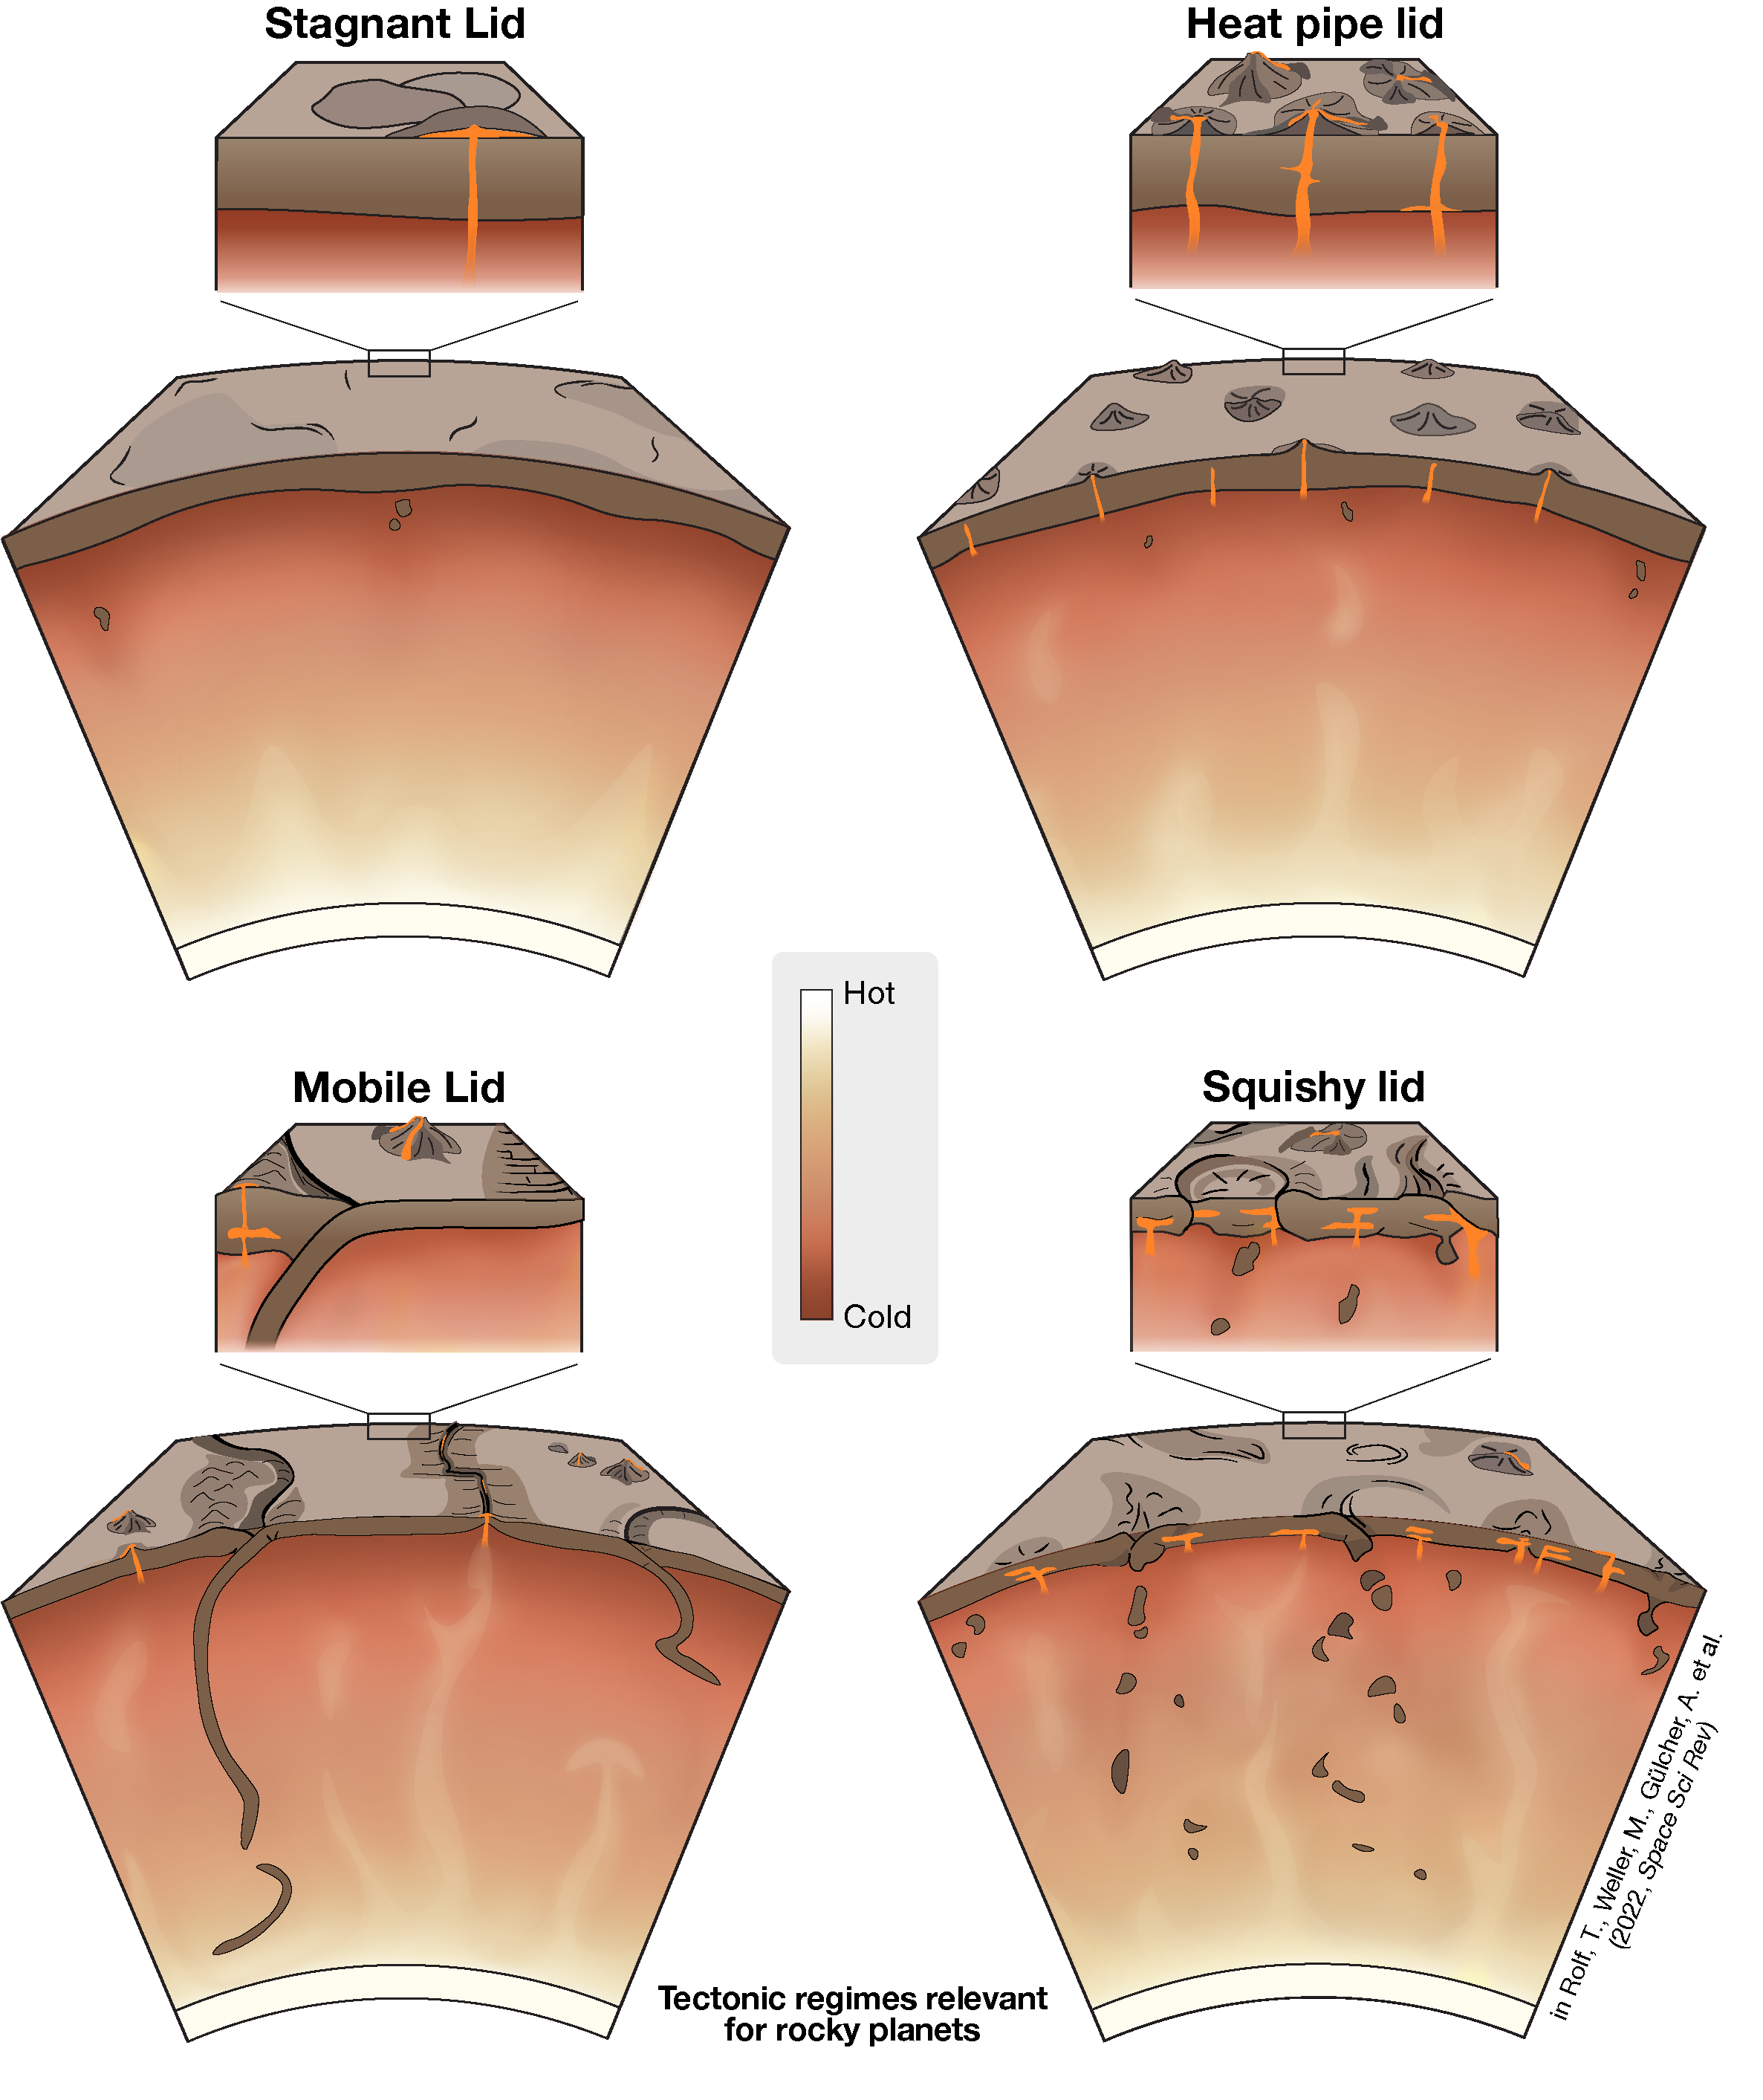
\includegraphics[width=\linewidth]{tectonic_regimes_AG}
\caption[Schematic of the four modalities of planetary tectonic style.]{Schematic of the four modalities of planetary tectonic style. See text for explanation. These graphics by Anna G\"ulcher from \citet{rolf_dynamics_2022} are available via the open-access s-Ink.org repository.}
\label{fig:tectonic_regimes}
\end{figure}



\subsection{Surface heat flow and tectonic mode}
\label{sec:intro-tectonicmode}

Tectonic ``mode'' or ``regime'' refers to the style of mechanical interaction between the outer, rigid layer of a planet and its convecting mantle. Where I have mentioned how the same parameterised model structure cannot arbitrarily be extrapolated to all geodynamic regimes \citep{seales_assessing_2019}, tectonic mode diversity is one of the most tangible reasons why rocky planets would be described by such different regimes. Four distinct tectonic modes are illustrated in Fig. \ref{fig:tectonic_regimes}. Stagnant lids are distinguished from mobile lids\footnote{Plate tectonics are a special case of mobile lids with highly localised deformation.} by how easily the lithosphere yields to plastic deformation---and hence can fail and subduct---whilst extreme cases of intrusive magmatism or extrusive volcanism can also alter  heat fluxes so much as to effect separate tectonic modes:
\begin{enumerate}
\item \textit{The stagnant lid mode} is associated with thick, insulating lithospheres that do not particpate in convection at all (Fig. \ref{fig:tectonic_regimes}, upper left).
\item Surfaces of planets in \textit{the mobile lid mode} move about as quickly as the mantle convects on average. The lithosphere participates in convection and is recycled into the mantle (Fig. \ref{fig:tectonic_regimes}, lower left). 
\item High rates of extrusive volcanism characterise \textit{the heat pipe mode}, with magma thought to pass through the lithosphere in narrow pipes, bringing down mantle temperatures (Fig. \ref{fig:tectonic_regimes}, upper right). This mode is thought to represent the extremely volcanic moon Io, and possibly many terrestrial planets whilst they are young \citep{moore_heatpipe_2013, moore_heatpipe_2017}.
\item \textit{The plutonic squishy-lid mode} also sees high rates of melting, although most of this melt does not extrude at the surface, instead remaining as warm, weak regions in the lithosphere. Denser mineral phases can then drip into the mantle (Fig. \ref{fig:tectonic_regimes}, lower right). This mode has been proposed for modern-day Venus, and could explain some of its observed surface deformation in absence of plate subduction \citep{lourenco_plutonicsquishy_2017, lourenco_efficient_2018, lourenco_plutonicsquishy_2020}.
\end{enumerate} 

A major effect of tectonic mode with regards to (parameterised models of) thermal convection is that it will modify the relationship between convective vigour and surface heat flux (the parameter $\beta$ in \eqref{eq:Ra-Nu}). This has consequences for internal cooling feedbacks, which I discuss in section \ref{sec:background-feedbacks}. Subduction of cold lithosphere is an efficient way to cool the mantle \citep{breuer_dynamics_2015}; so is volcanism, which is expected to be limited on stagnant lid planets with thick lithospheres  \citep{oneill_geological_2007, kite2009geodynamics, noack2014can, noack_volcanism_2017}. Hence stagnant lid planets will trap heat and run hotter, compared to those with mobile lids, for the same $R_p$. A related consequence is that the cores of stagnant lid planets might also cool inefficiently, weakening outer core convection and therefore the possibility of a geodynamo \citep{nimmo_why_2002, driscoll_thermal_2014}. 


Beyond heat transfer explicitly, tectonic mode is also an extremely important control on the chemical cycling between planetary surface and interior. Limited volcanism presents problems for the supply of fresh, weatherable surface rock, or atmospheric gases---a phenomenon explored in Chapter \ref{chapter:outgassing} of this thesis. Plate tectonics on Earth, meanwhile, with its dynamic outgassing of mantle water and subduction of hydrated crust, has helped stabilise the area of exposed continents for about half of Earth history \citep{kasting_what_1992, korenaga_global_2017, honing_longterm_2018}. Whereas subducting plates then carry surface material to the mantle, whether or not other regimes can close the circuit is unclear. We do not know how effectively planets without plate tectonics bury crustal carbonate to help regulate their atmospheric \ce{CO2}, for example \citep[e.g.,][]{elkins-tanton_volcanism_2007, foley_carbon_2018, honing_longterm_2018, honing_carbon_2019, honing_early_2021, rolf_dynamics_2022}. %The surface of stagnant-lid Mars appears to be billions of years old, implying that material has been stuck there for as long \todo{(REF)}. 




I highlight tectonic modes here because they are certainly something we will have to assume, at the moment, whenever we build a thermal evolution model. It is not currently possible to predict what mode a planet is in \textit{a priori} \citep{korenaga_plate_2012, lenardic_notion_2012, lenardic_solar_2016, weller_evolution_2018, ballmer_diversity_2021}; the case of Venus illustrates how this is difficult even having observations of the planetary surface in hand \citep[e.g.,][]{davaille_experimental_2017, rolf_dynamics_2022}. The literature is split between the stagnant lid or plate tectonics mode as the popular choice in model design. One reason to assume Earth-like plate tectonics in our models is that we already know this mode is able to sustain the geochemical cycles thought to stabilise the climate and support life as we know it. Yet because the physics of plate tectonics is also more complicated, the model implementation is less straightforward in practice (for example, one might need to assume the total length of subduction zones). Further, we have not settled on an explanation for why plate tectonics develops on certain planets (including on Earth!), whilst stagnant lids are widely reproduced in analogue laborarory settings and in numerical models, as discussed in the next section. In this thesis, I opt for the stagnant lid regime when I model planetary thermal evolution in Chapters \ref{chapter:topography} and \ref{chapter:outgassing}.


%relevant for thermal history because plate tectonics would somewhat decouple q_sfc from T_m --- because the mantle is ingesting cold lithosphere --- whilst stagnant lid lowers q_sfc for the same T_m - less efficient heat flux - compared to ``classic" Ra-Nu scaling thermal history model 






\subsubsection{The stagnant lid planet as a ``default'' mode}


Stagnant lids (Fig. \ref{fig:tectonic_regimes}, upper left) appear to be a natural consequence of temperature-dependent convection. Laboratory experiments observing scaled-down cells of convecting syrup show that if the viscosity increases sufficiently with decreasing temperature, the cold surface of the convecting cell will be so viscous as to not flow with the convection at all, forming a ``lid'' \citep{davaille_transient_1993, giannandrea_variable_1993}. Numerical experiments have replicated this behaviour at larger scales  \citep{solomatov_scaling_1995, moresi_numerical_1995, solomatov_can_1996}. Heat flows through the lid via conduction, while convection occurs only below the lid, where conditions are hotter and less viscous \citep{morris_boundarylayer_1984, christensen_convection_1984, hansen_high_1993, solomatov_scaling_1995}. Here, the stable stagnant lid is distinct from the upper thermal boundary layer, which is convectively unstable.

Silicate rock has a strongly temperature-dependent rheology \citep{karato_rheology_1993}. %, and indeed the Moon and Mars seem to behave as if they have a stagnant lid \todo{in what sense?}. 
In our own solar system, rocky planets are more frequently found in a non-plate tectonics regime than in a plate tectonic regime \citep{stern_stagnant_2018}. %This fact inspires many questions about whether stagnant lid planets can form ``continents" and other topographic complexities. The character of certain tesserae on Venus imply tectonic origin, questioning whether this world always had a purely stagnant lid \citep{Bindschadler1991, Lenardic1991}. 
The small-number statistics of the solar system bodies do not help much to answer how common plate tectonics is in the universe. Nevertheless, accepting the hypothesis, ``stagnant lids represent the default state of a planet'', might be more justified than applying Earth's plate tectonics to other planets, before we can explain why it began on our world in the first place. %In contrast, our theory of how stagnant lids develop is supported numerically and empirically.
%in justifying that until we know any better we can assume SL is at least plausible, which is perhaps more justifiable than assuming PT because Earth has it, since we can't explain why Earth has it but we can explain why other planets would have SL.}





%Maps of convective regimes in viscosity contrast-Rayleigh number space can be found in \citet{solomatov_can_1996} and more recently in \citet{huttig_regime_2011} and \citet{miyagoshi_thermal_2015}, with stagnant lids favoured by higher Rayleigh numbers \textgreater~$10^{6}$--10$^{7}$ and viscosity contrasts \textgreater~$10^4$ between the interior mantle and the surface.


%For practical reasons, this thesis considers a stagnant lid regime under the premise that it represents a ``default" rocky planet \citep{stern_stagnant_2018}. With the assumption of a stagnant lid we avoid some unknown complexities that mobile plates introduce. %Namely, plate margin-dominated heat loss on Earth works differently \citep[and more efficiently---stagnant lid planets will run hotter for the same rheology and surface heat flow;][]{stevenson_styles_2003} than in a stagnant lid regime, where heat loss is simply determined by boundary layer scaling laws like those we have discussed.


%\begin{figure}
%  \centering
%  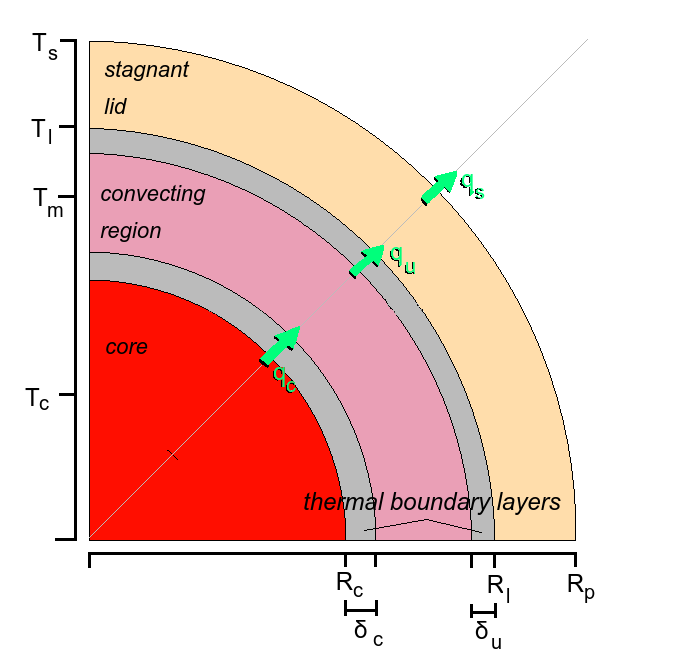
\includegraphics[width=0.5\linewidth]{stagnantlid}
%\caption{Structural model of a stagnant lid planet, not to scale. $R_p$ is the radius of the planet, $R_l$ is the radius at the base of the lid, $R_c$ is the radius of the core, $T_s$ is the surface temperature, $T_l$ is the temperature at $R_l$, $T_m$ is the isothermal convecting cell temperature, $T_c$ is the isothermal core temperature, and $\delta_u$ and $\delta_c$ are the upper and lower thermal boundary layer thicknesses respectively. The boundary layer heat fluxes $q_c$ and $q_u$ and the surface heat flux $q_s$ are defined in equations (\ref{eq:q_Ra}) and (\ref{eq:q_s}), respectively}. 
%\label{fig:stagnant_lid}
%\end{figure}




%
%\subsubsection{The solar system's tectonic garden}
%
%Stagnant lids are differentiated from mobile lids\footnote{Plate tectonics are a special case of mobile lids with highly localised deformation}) by how easily the lithosphere yields to plastic deformation \citep{rolf_dynamics_2022}. I have mentioned that stagnant lid planets cool inefficienlt because
%in the stagnant lid regime, heat conducts ineffiecinetly through the lid because it is so thick. However, planets can also lose heat by magmatism, and even planets with low-velocity lids can have magmatic styles that are different enough to put them into another tectonic regime. The heat pipe regime is characterised by high rates of extrusive volcanism, with magma thought to pass through the lithosphere in narrow pipes.}
%
%
%
%\todo{Other regimes ... heat pipe and squishy lid... newer. kind of cool in between that does involve some chemical interaction via plutonism. believed for venus. they avoid one of the possible issues of true stagnant lids in nature which is that they would be really hot maybe too hot because inefficient heat loss. stuff probably wants to melt!}
%





\subsection{Planetary self-regulation and determinism}
\label{sec:background-feedbacks}
% if this section is here then tie to beta in Ra-Nu relationship. positive beta implies feedback, convective vigour and heat loss are coupled. smaller beta imples more decoupled, negative beta has been suggested for PT..

Inherent to the thermal history of planets, and indeed recognised since the first convection models, are the dynamic feedbacks that regulate mantle temperatures over geologic time. The presence of these feedbacks will be implicit to the results of Chapters \ref{chapter:topography} and \ref{chapter:outgassing}. %\todo{in such a way that makes predicting them a lot more viable.} 
\citet{lenardic_internal_2022} argue that feedback loops in mantle convection deserve just as paradigm-shifting a status as the Daisyworld of climate homeostasis \citep{lovelock_atmospheric_1974, watson_biological_1983}, or of course \citeauthor{walker_negative_1981}'s (\citeyear{walker_negative_1981}) silicate weathering thermostat. That is, in much the same way as feedbacks which stabilise surface temperatures prolong the ``habitable lifetime'' of a planet, feedbacks which stabilise mantle temperatures will also prolong the geodynamic lifetime of a planet. The possibility of mantle self-regulation should also be of strong practical interest to exoplanet researchers because it entails that mantles will lose the memory of their initial state, such that---from a modelling standpoint---much of the stochasticity inherent in forming planets can be removed. Understanding these feedbacks might help us judge whether certain phenomena of Earth are likely a fluke of thermal history \citep[e.g., the fact that the temperature near the top of the mantle is very close to the melting temperature of peridotite;][]{seales_buffering_2022}, or if these phenomena are also representative of other planets. At the same time, feedback loops can be a double-edged sword if they lead to multiple stable solutions for a planet's evolution---perhaps Earth and Venus followed diverging paths from simiar initial conditions \citep{lenardic_solar_2016}.

The most fundamental feedback regulating thermal evolution follows from the temperature-dependence of mantle viscosity \citep{tozer_present_1972}. Decreasing temperature raises viscosity, which leads to less vigorous convection, and less heat flow out of the mantle, which in turn heats the mantle and lowers its viscosity. This feedback would buffer the interior at a near-constant viscosity, even as its internal heating rate decreases with exponential radionuclide decay, a corollary of which is a narrow range of mantle viscosities for rocky exoplanets. This \citeauthor{tozer_present_1972} feedback has not been proven to occur on Earth, hence it is not guaranteed to occur on other planets either \citep{korenaga_can_2016}; its efficiency depends on whether the heat flux out of the mantle can adjust quickly enough to a change in temperature. Parameterised models capture response time via the $\beta$ parameter in \eqref{eq:Ra-Nu}, for which the classic value of 1/3 corresponds to quick response time and self-regulation \citep{seales_assessing_2019}.

Theory suggests that stagnant lid convection ($\beta \approx 1/3$) should always meet this short thermal response requirement, at least on an Earth-mass planet \citep{korenaga_can_2016}. Less is understood about the rheological behaviour of rock at the several-hundred-GPa pressures found in planets more massive than Earth, but we would at least expect viscosity to increase with pressure \citep{christensen_convection_1984}---the strength of the pressure-dependence may preclude viscosity self-reguation \citep{stamenkovic_influence_2012}, or may not \citep{tackley_mantle_2013}. As for planets with plate tectonics, $\beta$ depends on the extent to which plate motions are governed by mantle convection \citep[as opposed to, e.g., the plates' own strength;][]{conrad_effects_1999, crowley_analytic_2012}; $\beta$ here could be 0 or even negative \citep{korenaga_energetics_2003}. The parameterised convection model I use in Chapter \ref{chapter:topography} considers stagnant lid convection heated from below with $\beta \approx 1/3$.
%other feedbacks exist and are reviewed in lenardic & seales. 



%\todo{In any case the Earth controversies are useful to us now because they emphasise how low Ur (non thermally self-regulated ) systems can't exist  with  classical or stagnant lid style heat loss}

%\todo{The above argument also points out that classical models which are tuned to earth are actually wrong in that they don't even meet earth's constraints. so would be careful to do this. is there an example? like turcotte 2002 etc. better to use stagnant lid model with semi-empirical scalings?}


In any case, the generally-high thermal inertias of mantles means that with the natural decay of an internal heat source, they never do reach true thermal steady state \citep[cf.][]{tozer_present_1972}. Rather, planets cool down, perhaps in a series of quasi-steady states, until geodynamic death (no energy for mantle convection)---if they are not first swallowed in their star's asymptotic giant branch stage, that is. All planets therefore have a natural end to their convective, tectonic, and volcanic activity, possibly foretold by the size and heat-producing element budget with which they are born \citep{stevenson_styles_2003, frank_radiogenic_2014, unterborn_mantle_2022}. Luckily, these two parameters could be amenable to observation \citep{nimmo_radiogenic_2020, wang_europium_2020}. In this way it should be sensible to estimate the thermal histories of generic stagnant-lid planets.


























%
%\subsection{Two consequences of heat transport}
%
%\todo{In this thesis are two direct explorations of mantle thermal convection controlling surface properties}
%
%\subsubsection{The shapes of planets}
%
%\subsubsection{Volcanism and volcanic outgassing}












\section{Geology in the cosmos}
\label{sec:background-composition}
Section \ref{sec:background-thermalhistory} has presented the tools used to assess how planets evolve thermally over billions of years. Here I discuss what sets planets' material properties---properties which, in a pragmatic sense, will go into these thermal history models, but should also, in a broader ontological sense, influence the \textit{geologic} evolution of planets in complex ways we are just beginning to formalise. Namely, planets' interior compositions add another axis to their potential diversity. By ``composition'', exoplanet researchers can be referring to the first-order concentric structure of a planetary interior---the relative sizes of metallic, silicate, and volatile layers---as well as to higher-order concerns, such as abundances of specific elements or minerals in the mantle. The bulk element composition a planet inherits from its formation, in terms of the major rock-forming refractories but also volatiles like H and C, sets up its subsequent thermal evoluton via composition-dependent properties (e.g., viscosity parameters, solidus temperatures, oxidation state) and boundary conditions. Planetary differentiation---the segregation of iron and siderophile elements as a metal core to a planet, and the partial melting of a mantle forming a crust enriched in incompatible elements---means that these inherited elements become heterogeneously distributed within a single planet. Nevertheless, as I introduce throughout this section, inter-planet compositional diversity need not be infinite in every way despite the high entropy of the universe.

To the first order, the interior composition of a planet is linked to its bulk density: metal is denser than silicate, which is denser than ice or gas. When observers try to piece out the interior structure of a given exoplanet, however, they are blocked by a certain degeneracy: density provides two data in the planet mass and radius, but there are at least three possible compositional layers in a metal core, silicate mantle, and volatile envelope. A larger core, thinner mantle, and thicker volatile envelope would produce the same density as a smaller core, thicker mantle, and thinner volatile envelope. There is additional degeneracy from the possibility of a planet's silicate portion to be molten, if hot enough \citep[inducing $\sim$10\% density variations;][]{bower_linking_2019}, and less so, from the fact that the iron core could contain an unknown proportion of light elements such as Si and O \citep{unterborn_scaling_2016}. This degeneracy is the famous major problem of exoplanet interiors in the observational community. Such degeneracies prohibit a clean identification of water-poor, rocky planets (note Earth is water-poor, with its surface oceans contributing just $\sim$200~ppm of its mass). For example, four of the roughly Earth-mass planets orbiting the TRAPPIST-1 star, which appear to be $\sim$10\% less dense than Earth, could consequently have water mass fractions between $\sim$0--10\% depending on their unknown core sizes \citep{unterborn_inward_2018, agol_refining_2021}---enough water to preclude any dry land, as I show in Chapter \ref{chapter:topography}. 

I am mentioning this astrophysical barrier first because \textit{(i)} it is a good example of the limits to current knowledge from specific exoplanet observations alone, and \textit{(ii)} the reader should understand what this thesis is not aiming to resolve. Precise predictions for individual planets need not be our focus---although contributions from Earth science will certainly be needed to gather other constraints on planets' metal core sizes (section \ref{sec:background-redox}). For example, I am not interested in exoplanet chemical compositions for the sake of \textit{identifying} known planets as ``Earth-like'' or not, since I believe that such categories, which necessarily rely on a few state variables, are only ever going to mislead. To that end, higher-order mantle mineralogy, which in general does not lead to serious bulk density differences \citep{dorn_can_2015, unterborn_scaling_2016}, would not seem as important for interpreting the astrophysical mass-radius observations;\footnote{\citet{dorn_new_2019} present an exception: planets that are hypothetically rich in high-temperature condensates Ca and Al, for example because they form \textit{in situ} very close to their star, would be noticeably (10--20\%) less dense than Earth or Venus.} many astronomers are happy to consider mantles as pure \ce{MgSiO3} as such. The converse is that because mineralogical diversity is largely unrelated to bulk densities---and indeed, this diversity is best inferred by other observational means (the next section)---studies of exoplanet mineralogy are freed from the above degeneracy.


The fairly recent illumination of the rocky exoplanet composition axis is unforaged ground for researchers. That is, it opens new ways to approach the Big Question,\footnote{Are we alone?} and new needs for experimental work. Mantle mineralogy must surely be a consequential %\textit{and constrainable} 
state variable in the comparative thermochemical evolution of planets. The minerals stable through a mantle will affect, for example, its rheology \citep[e.g.,][]{spaargaren_influence_2020}---but in contentious directions \citep[ferropericlase may be stronger or weaker than bridgmanite; cf.][]{yamazaki_mineral_2001, cordier_periclase_2023}---its melting temperatures \citep[alkalis, Fe, and higher Ca/Al ratios depress the solidus;][]{hirschmann_mantle_2000, kiefer_effects_2015, brugman_experimental_2021}, and its volatile budget (Chapter \ref{chapter:rockywater}, this thesis). For a given geotherm, they will determine crust compositions \citep[e.g.,][]{fortin_volcanic_2022}: pyroxenes and quartz melt at lower temperatures, suggesting thicker crusts \citep{lambart_role_2016}, as do FeO-rich compositions in general \citep{dyck_effect_2021, wade_divergent_2017}. Crusts, being the result of extra processing, have much more geochemical complexity (i.e., less modelling tractability) than mantles, but are worth some more elaboration here. Their variable thickness brings still more complexity to the previous section's thermal history concepts: \textit{(i)} U, Th, and K are incompatible such that thicker crusts remove more heat-producing elements from the mantle; and \textit{(ii)} crusts can reduce conductive heat loss \citep{lenardic_continental_2005, lenardic_note_2011}. Less understood but very important is how crust composition could affect the tectonic regime, given that some lithologies will be more deformable \citep[lower yield stress to plate formation; e.g.,][]{karato_remarks_2014, weller_evolution_2018, ballmer_diversity_2021}. %, whilst thick basaltic crusts could also self-destabilise if they reach eclogite transition pressures \citep{orourke_terrestrial_2012}---there is a complex relationship between mantle mineralogy, crust composition and thickness, and lithosphere strength. 
Dimensions like these are worth pursuing not only for curiosity reasons  \textit{(what kinds of planets could be out there?)}, but also because understanding what planets are capable of without life is necessary for attributing biologic origin to any signal \citep{wordsworth_redox_2018, lisse_geologically_2020, krissansen-totton_oxygen_2021, krissansen-totton_understanding_2022, butkus_note_2023}.



One community which has shown itself as incredibly well-poised to help understand exoplanet geology is that of the theoretical mineral physicists. The existence of a large population of massive rocky planets implies the existence of mantle rocks at extremely high-pressures: up to $\sim$630~GPa at the core-mantle boundary, versus 136~GPa on Earth \citep{unterborn_pressure_2019}. As such, research into Earth's deep mantle naturally extends to exoplanets. Density functional theory, \textit{ab initio} molecular dynamics, and machine learning have been vital in predicting the high-pressure material propreties---particularly, rheological and melting properties---of known lower mantle phases like postperovskite and ferropericlase \citep[e.g.,][]{tackley_mantle_2013, stixrude_melting_2014, millot_shock_2015, sakai_experimental_2016, ritterbex_vacancies_2018}, but also the alien mineral phase transitions that occur beyond postperovskite \citep[e.g.,][]{umemoto_twostage_2011, umemoto_phase_2017, coppari_implications_2021}. Theoretical equations of state of postperovskite agree very well with experimental data up to $\sim$300~GPa, for example \citep{sakai_experimental_2016}. These high-pressure mineral properties and phase diagrams are currently a source of uncertainty in comparative planetary evolution research---but with this discipline's enthusiastic pace, we might soon approach the limit of what is technologically possible to constrain.




\subsection{The chemical diversity of stars (and their planets)}
\label{sec:background-starchem}
% in this section should actually say what some of these are... maybe with ternary diagram?

The crux of rocky planet composition insight is that planets are chemically linked to their host stars. A star and its planets grow from the same nebular cloud; stars contain \textgreater 99\% of the mass, so their elemental compositions---which are spectroscopically observable---are a good proxy for those of the nebula. Most atoms in stars may be hydrogen or helium, but if we remove these and consider only the major rock-forming, refractory elements (Mg, Si, Fe, Ca, and Al), then is it not likely the condensing building blocks of planets inherit the same relative inventory of these elements? This behaviour exactly has been replicated in planet formation simulations \citep{bond_compositional_2010, thiabaud_elemental_2015} and is consistent with an observational pilot study \citep[discussed below;][]{bonsor_hoststar_2021}. If true, then the measureable compositional diversity of stars---the variability in their refractory element ratios---may therefore inform the compositional diversity of planets. 

Namely, main sequence stars have different element abundances because they form in different parts of the galaxy with their own local chemical evolution \citep{hinkel_stellar_2014}, but not \textit{too} different because they still obey the same rules of nucleosynthesis \citep{burbidge_synthesis_1957}: they will always contain greater abundances of Si, Mg, and Fe, for example, than Ti and Cr (being other, minor rock-forming elements). The releative proportions of refractory elements determine which mineral phases are stable as a function of temperature and pressure in the mantle. Simple stoichiometry tells us that increasing Mg with respect to Si favours forsterite (the olivine endmember \ce{Mg2SiO4}) over enstatite (the orthopyroxene endmember \ce{MgSiO3}) because the former takes two Mg atoms per Si atom. I use this example because Mg/Si has the largest effect on modal mantle mineralogy---and hence is quoted sometimes as a proxy---because Mg and Si are the most common elements is silicate rocks apart from oxygen. In the Hypatia Catalog of nearby FGKM stars, 68\% of measurements show Mg/Si between 0.91 and 1.35 \citep{hinkel_stellar_2014}; i.e., most rocky planets are pyrolitic. That planet-hosting stars have minor variations in their element abundances is a major premise of the second half of this thesis. 



When stellar element abundances are used to estimate exoplanet mantle mineralogies, wholly foreign compositions (with respect to the solar system) do not appear \citep{hinkel_star_2018, putirka_composition_2019, wang_enhanced_2019, wang_detailed_2022, spaargaren_plausible_2022}. Given the broad consistency between stellar abundance patterns, phase equilibria modelling produces only a handful of mineral phases stable at mantle conditions: olivine polymorphs, pyroxenes, spinel, and garnet in the upper mantle, and (post)perovskites and ferropericlase (also known as magnesiow\"ustite) in the lower mantle, with possible silica phases (quartz, coesite, stishovite) stable in the most Si-rich cases. The exception is in the deep lower mantles of $\sim$4-Earth-mass planets and up, where \ce{MgSiO3} postperovskite has been predicted to recombine into new phases above $\sim$0.5 TPa \citep{umemoto_phase_2017}. Robust predictions of these high-pressure mineral phase equilibria are only as good as the thermodynamic (theoretical and experimental) data. Yet our datasets are always expanding, such as the thorough, probably painstaking compilation of \citet{stixrude_thermal_2022}, which accounts even further for the realistic thermodynamics of solid solutions.\footnote{For example, in the \citet{stixrude_thermal_2022} dataset, the ``perovskite'' phase is a solid solution of \ce{Al2O3}, \ce{FeSiO3}, and \ce{MgSiO3}.} Chapter \ref{chapter:rockywater} demonstrates how to predict self-consistent phase proportions, adiabatic profiles, and mass-radius relationships for arbitrary (but plausible) refractory compositions of planets up to about 4 Earth masses, before the phase equilibria uncertainties might start to challenge our trust.
%In absense of very extreme partitioning scenarios, these nucleosynthesis patterns mean that we do not expect graphite/diamond planets, aluminium planets, \textit{etc.} to exist \todo{(REF?)}.
% cf. madhu 2012 ApJL, born
% can't find formation model precluding carbon planets... wilson+ 2016 find no evidence  for C-rich planetary material from PWD C/O measurements, also jura & young review says this, but haven't introduced WDs yet at this point


%Out of the various element ratios, Mg/Si has the biggest effect on modal mineralogy---hence it is quoted sometimes as a proxy---because Mg and Si are the most common elements is silicate rocks apart from oxygen. Simple stoichiometry tells us that increasing Mg/Si favours forsterite (the olivine endmember \ce{Mg2SiO4}) over enstatite (the orthopyroxene endmember \ce{MgSiO3}) because the former takes two Mg atoms per Si atom. %If Mg/Si $\gtrsim$ 1.5 then no orthopyroxene stabilises; whilst if Mg/Si $\lesssim$ 0.7, there is no stable olivine, and the excess Si will form silica phases. Compositions richer in Al will stabilise more spinel and garnet, although aluminous phases are not expected to make up more than half the mass in the olivine stability field. 


% [What stoichiometry is Si-limited to make olivine and where does that Mg go?],

% therefore broadly get the same minerals as in earth, which thermodynamic phase diagrams (plus simple stoichiometry) show us are the stable phases:  




% Mars Mg/Si=0.88 (Yoshizaki & McDonough 2020)
As I write this, the preservation of refractory ratios between planet and star remains a \textit{fundamental assumption} and a \textit{working hypothesis}. The solar photosphere's measured Mg/Si ratio (1.05), whilst virtually exactly the same as CI chondrites within error, notably underestimates the value of 1.27 canonical for Earth's upper mantle \citep{ringwood_significance_1989, palme_solar_2014}. A robust explanation of this misfit would close a conspicuous knowledge gap in exoplanet research. It is conceivable that our models of the Bulk Silicate Earth composition are simply not sampling the entire mantle, insofar as they are based on upper mantle xenoliths \citep{matas_bulk_2007, javoy_chemical_2010}, though some analyses have argued against this \citep{lyubetskaya_chemical_2007a}. However, Mg and Si also could have relatively fractionated through a dynamic process as the Earth and other planets accreted, despite the 30-K difference in their 50\% condensation temperatures \citep{ringwood_significance_1989, miyazaki_dynamic_2020}. Even more likely is that some Si enters the metal core and is trapped there \citep{ringwood_chemical_1959, javoy_integral_1995, Wood2006, schaefer_metalsilicate_2017}; some estimates of Earth's core Si content are up to $\lesssim$10 wt.\% \citep{wade_core_2005, ricolleau_oxygen_2011, fischer_high_2015}.  

%how Si partitions into cores and if we can estimate this, which not only affects core densitt as above but also mantle composition, and other processes that partition si with respect to major refractory elements like Mg in the protoplanetary disc (e.g. miyazaki), and how volatiles are delivered to planets?.


As to be expected, the volatile element abundances of planets are much more removed from those of their host stars. Rather than condensing at high temperatures near the centre of the protoplanetary disc, these elements will be transported to the disc's outer regions \citep{ringwood_significance_1989, cassen_models_1996, ciesla_radial_2008}. However, volatiles can then be scattered inwards from gravitational perturbations, and whole planets can also migrate \citep[e.g.,][]{unterborn_inward_2018, raymond_migrationdriven_2018}. Oxygen is a particular nuisance because it can be dually refractory (bound up as oxide components of rocky material; e.g., as \ce{SiO2}) or volatile (e.g., as \ce{H2O}), and Earth's total oxygen budget has not yet been explained unamimously in terms of its stochastic accretion \citep[e.g.,][]{raymond_making_2004, morbidelli_building_2012, rubie_accretion_2015, obrien_delivery_2018, sossi_stochastic_2022}. Further, moderately-volatile alkalis such as Na and K, whilst relatively unimportant for a mantle's mineral proportions, can be quite consequential for its melting behaviour \citep{hirschmann_mantle_2000}. \citet{wang_detailed_2022} make a good start using empirical star-planet depletion trends, based on our solar system, to estimate rocky exoplanet mantle compositions; in Chapter \ref{chapter:fo2} I will take a similar approach when estimating planets' Na compositions. Nevertheless, we do not have the data to evaluate whether this solar system trend is the best model for planetary systems in general. Major theoretical questions linger over the degree to which the ingredients of extrasolar rocky material deviate from stars; an answer begs a good understanding of high-pressure metal-silicate partitioning behaviour and the dynamic chemical evolution of protoplanetary discs.

% Hinkel & Unterborn 2018:
% In general, the error reported for stellar abundances of [Mg/H], [Al/H], [Si/H], and [Ca/H] are 0.07 dex, 0.06 dex, 0.05 dex, and 0.06 dex, respectively (Hinkel et al. 2014). 
%Nissen (2015) reported errors of 0.009 dex, 0.005 dex, 0.005 dex, and 0.006 dex, while Spina et al. (2016) had errors of 0.014 dex, 0.012 dex, 0.007 dex, and 0.013 dex. 

Errors in both planet bulk densities and host star abundances limit predictions about the interior composition of a given planet. In particular, the typical measurement error on individual host star abundances \citet{hinkel_star_2018} propagates to an error on Mg/Si of $\sim$0.2: nearly consuming the Sun-Earth Mg/Si discrepancy. The more problematic type of uncertainty, however, is the spread in reported values between the various techniques used to retrieve abundances from the raw stellar spectra \citep{hinkel_comparison_2016}. A thorough discussion of error propagation from stellar abundances to exoplanet mineralogy can be found in \citet{hinkel_star_2018}. As per the theme of this chapter, what remains tractable is the \textit{range} of stellar refractory ratios, which should inform the minimum \textit{range} of planet refractory ratios, so long as their fractionation processes are minor and roughly universal across protoplanetary discs \citep{bond_compositional_2010, thiabaud_elemental_2015}. (It is already interesting to note that the Sun is very close to the median in terms of Mg/Si/Fe.) From here, the field looks wide open for us to explore and eventually formalise the many ways mineralogy, inherited at birth, determines planet evolution. % very new. lots of experimental petrology work to be done such as the solubility of volatiles (water and carbon) in different mantle rock types (e.g. sossi). 
\citet{spaargaren_influence_2020} have bravely started incorporating mantle mineralogy into thermal evolution models; we are no longer confined to canonical Bulk Silicate Earth as representative of all exoplanet mantle compositions. To model these evolutions most effectively, however, we need more experimental and \textit{ab initio} data on rock viscosities and melting temperatures across the diversity of mantle mineralogies we now expect.  




\subsubsection{More clues from stellar remnants}
\label{sec:background-pwd}



\begin{figure}
  \centering
  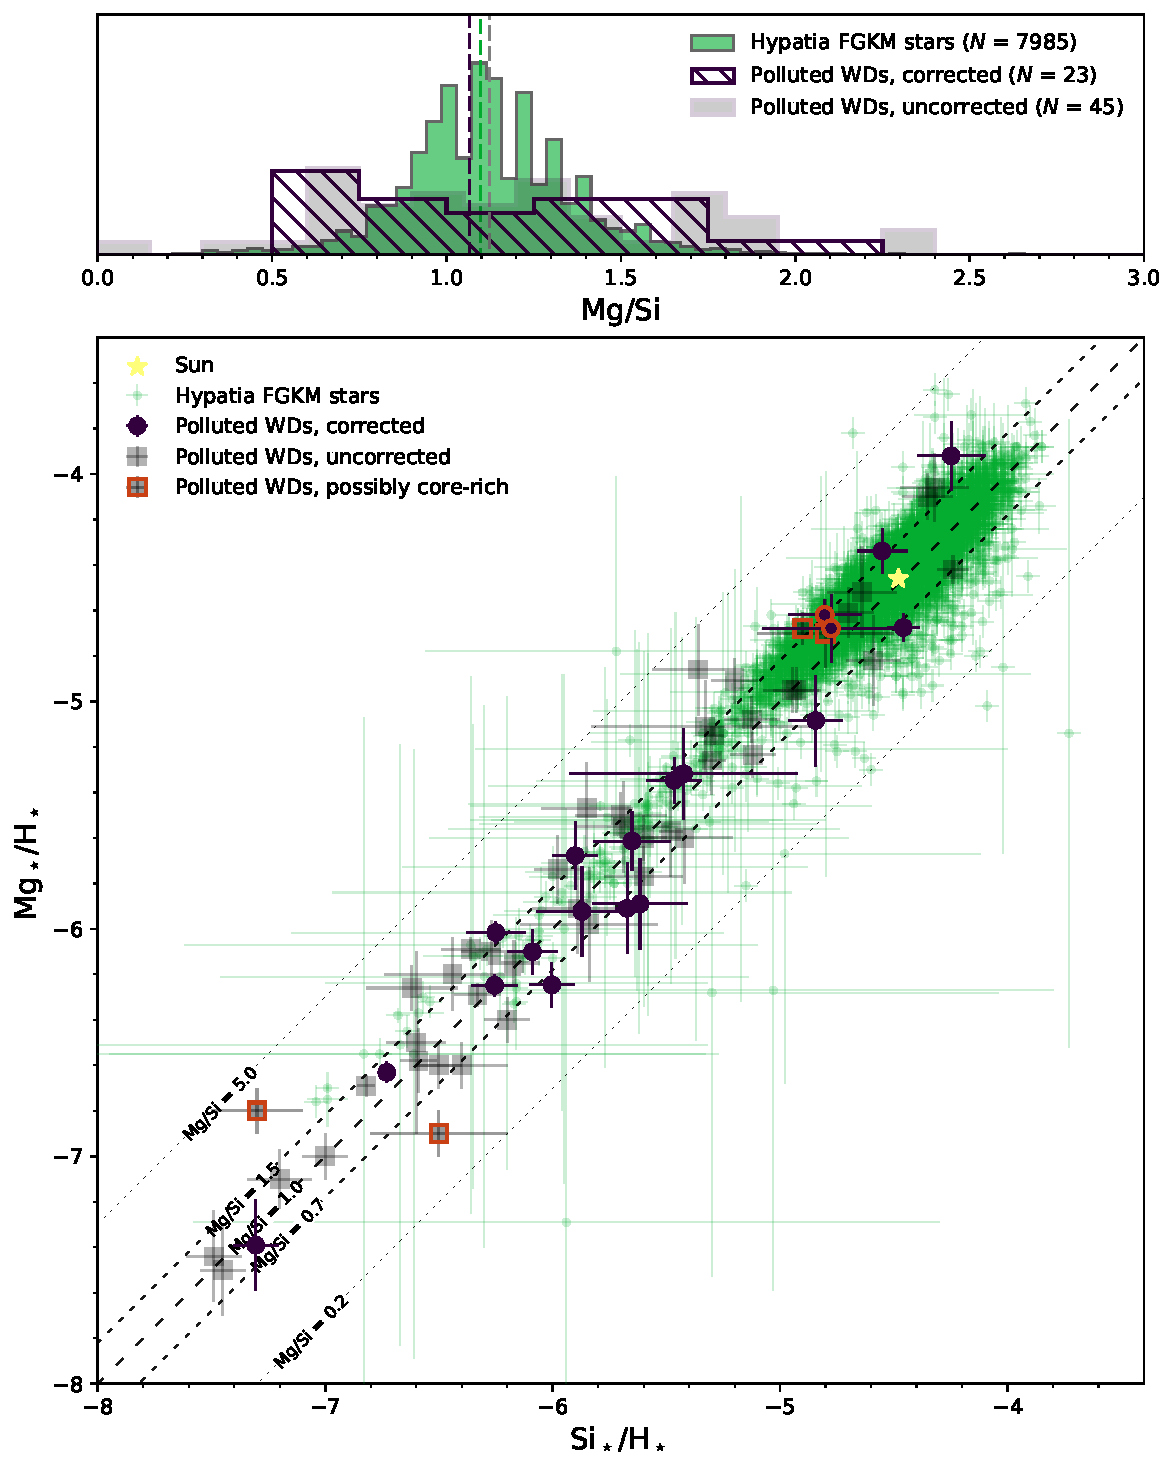
\includegraphics[width=0.95\linewidth]{wd_hypatia_mgsi.pdf}
\caption[Comparing Mg/Si ratios between FGKM stars and polluted white dwarfs, which provide independent constraints on rocky exoplanet bulk compositions.]{Comparing Mg/Si abundances between FGKM stars and polluted white dwarfs (WDs), which provide independent constraints on rocky exoplanet bulk compositions. \textit{(Bottom:)} Observed stellar abundances with respect to H, where the number ratio ${\rm X}_\star/{\rm H}_\star = \log_{10}(n_X/n_H)$ in astronomical notation (note abundances are not solar-normalised). The green dots show all FGKM stars in the Hypatia Catalog$^a$ with measured Mg and Si at time of writing. WD data are from a compilation provided by Andrew Buchan (including unpublished data from Laura Rogers), where the purple circles have been corrected to steady-state accretion by accounting for differential sinking; grey squares are uncorrected; and the points highlighted orange are likely to be core-rich fragments (estimated core mass fraction $> 0.4$). The errors on both data sets are different: the Hypatia Catalog reports errors as the spread between different sets of measurements---which can be quite high---whilst the WD errors are the measurement uncertainties as reported in the original publications. The typical measurement uncertainties of the Hypatia abundances are 0.07 dex for ${\rm Mg}_\star/{\rm H}_\star$ and 0.05 dex for ${\rm Si}_\star/{\rm H}_\star$ \citep{hinkel_stellar_2014}. Diagonal lines denote reference molar ratios: above ${\rm Mg/Si} \approx 1.5$, orthopyroxene disappears from the upper mantle, and below ${\rm Mg/Si} \approx 0.7$, pure-\ce{SiO2} polymorphs become stable throughout. \textit{(Top:)} Histograms of the same data, The vertical dashed lines show the medians.\\ 
\vspace*{10.5em} \footnotesize{$^a$\citet{hinkel_stellar_2014, hinkel_comparison_2016}, https://www.hypatiacatalog.com/}
}
\label{fig:hypatia_vs_pwd}
\end{figure}
%\todo{[todo: find out from Andy which are optical vs UV!]}

There is an independent way to probe (disintegrated) planet compositions through (the afterlives of) stars. Well-established stellar evolution concludes in white dwarfs, stars' collapsed, electron-degenerate remains. White dwarfs are so dense that their photospheres should only contain H or He---the temporary presence of any heavier element would seem to have exogenous origins. We now believe that the exogenous material represents planet(esimals), asteroids, or exomoons from the outer regions of an ancient planetary system,\footnote{i.e., because the star would have engulfed anything within an AU or so during its asymptotic giant phase \citep{veras_postmainsequence_2016}.} ripped apart by tidal forces, and eventually accreted onto the white dwarf \citep{jura_extrasolar_2014}. At least a third of observed white dwarfs are ``polluted" as such \citep{koester_frequency_2014}. Because heavy elements sink through white dwarf photospheres in less than 0.1 Gyr \citep{koester_accretion_2009}, the pollution must have been recent, in astronomical terms---the accretion event itself could be as short as years \citep{rogers_nearinfrared_2020}---and it is commonly assumed that each observed assemblage of pollutants represents a single body: a complete parent body, or post-collisional fragment of \citep{jura_extrasolar_2014}. Observations of heavy element abundances in polluted white dwarfs therefore provide a direct probe into exoplanetary system compositions.


Compared to main sequence star abundances, the measurement uncertainty here is typically higher because the spectral lines of white dwarfs will necessarily have higher gravitational broadening \citep[e.g.,][]{bonsor_hoststar_2021}. Further, a fair amount of modelling is needed if we are to infer parent body and particularly exoplanet compositions from white dwarf photosphere abundances \citep[e.g.,][]{harrison_polluted_2018, harrison_bayesian_2021, buchan_planets_2022}. Any estimation of exoplanet compositions from polluted white dwarfs would want to consider two complications:
\begin{enumerate}[label=(\roman*),font=\itshape]

\item Not much is known \textit{a priori} about the nature of the individual accreted bodies that our measurements are sampling: their mass, degree of metal-silicate differentiation, and---if collisional fragments---the degree to which they contain the parent body's core or silicate mantle, analogous to iron meteorites, stony achondrites, and pallasites from our solar system \citep{bonsor_are_2020, buchan_planets_2022}. However, geochemical constraints such as pressure- (size-) dependent element partitioning may be leveraged to this end \citep{buchan_planets_2022}.

\item Different elements sink at different rates through white dwarf photospheres. These rates depend on the white dwarf's effective temperature, surface gravity, and whether it is H- or He-dominanted; interpreting the observed abundances hinges on whether the accretion is in an ongoing, declining, or steady-state phase \citep{jura_extrasolar_2014}. \citet{brouwers_asynchronous_2023} showed that accretion-timeline uncertainties create artificial variation in inferred parent body oxygen contents. Oxygen sinks relatively slowly, so observing it in excess could actually mean that the accretion event happened a long time ago, rather than that the parent body was O-rich. 

\end{enumerate}
Neglecting these complications may lead to less-significant or possibly misleading results. Accounting for effects \textit{(i)} and \textit{(ii)} may question the number of O-rich white dwarfs reported in \citet{doyle_new_2023}, for example. %Chapters \ref{chapter:rockywater} and \ref{chapter:fo2} sidestep these complications by focusing on the main sequence stars' indirect constraints on exoplanet compositions (opting instead to be hindered by the other complications from section \ref{sec:background-starchem} therein). 

With uncertainties accounted for, observations of polluted white dwarfs can not only clue us to exocosmochemical variability, they can also help corroborate our earlier presupposition that planet refractory ratios equal star refractory ratios. This is possible because white dwarfs provide an independent constraint. \citet{bonsor_hoststar_2021} compared the refractory element composition of the polluted white dwarf WD 1425+540 with its K-dwarf binary pair G200-40 (expected to be chemical twins), showing that the pollutant and G200-40 compositions were alike within error, whilst they differed from a random K-dwarf. Increasingly precise observations of polluted white dwarfs, combined with theoretical developments in how they accrete rocky material, will likely prove invaluable if we want believable constraints on the mineralogy of specific nearby exoplanets.

We can start to make preliminary comparisons between the refractory variability of polluted white dwarfs versus FGKM stars. Figure \ref{fig:hypatia_vs_pwd} shows this comparison for Mg and Si. Polluted white dwarfs appear to show greater dispersion in Mg/Si than the FGKM stars, reflecting the fact that the former measurements sample a range of planetary material which has variously differentiated, fragmented, and otherwise been processed. However, the distribution medians seem very similar (1.10 vs. 1.09 or 1.12 depending on correction). Similar medians would suggest that, on average, the formation and evolution of planets is not systematically fractionating Mg/Si---and hence the proportions of major mantle elements---in a particular direction.




% figure comparing mg/si and mg/fe in WD vs hypatia planet-hosting?

%I think there's an even more fundamental issue which is that (as far as I can tell) they don't consider the possibility of accretion being in declining phase, which is huge. Oxygen generally sinks slowly, so an apparent excess of oxygen could also just be explained by the accretion having already ended a while ago, and everything else has just sunk faster through the white dwarf atmosphere, so you really need to take this into account. (This is one of the key points from this paper https://arxiv.org/abs/2211.05113 ). (They also don't seem to consider the possibility of differentiation + fragmentation, although that's less fundamental). I reran this systems with my model - according to my model only one of these systems (0218) is actually likely to have an oxygen excess. - Andy


\subsection{The importance of core size, and attempts to constrain it}
\label{sec:background-redox}
% keep this section very short because it could be a rabbit hole lol

To complete the circle, there is a useful future role for Earth science in interpreting planet composition constraints, for the purpose of ameliorating the ruesome bulk density-interior structure degeneracy (section \ref{sec:background-starchem}). Because this degeneracy exists due to unconstrained metal core sizes, geochemical limits to core formation may therefore offer some insight into exoplanets' interior structures. Metal cores form according to the equilibrium:
\begin{equation}
\label{eq:background-iw}
\ce{Fe^{\rm metal} + \frac{1}{2} O2 <=> FeO^{\rm silicate}}.
\end{equation}
Here, iron is undergoing redox reactions within young planets' magma oceans---the stage during which planets are so hot from accretion energy and short-lived radionuclides to be largely molten \citep{elkins-tanton_magma_2012}---where the dense metallic iron eventually sinks to the planet centre \citep{kleine_rapid_2002, yin_short_2002, wade_core_2005, Wood2006}. Importantly, equilibrium \eqref{eq:background-iw} need not go to completion. Some FeO could remain in the mantle such that the final core mass fraction will be related to the molar ratio of Fe-metal to FeO, $X_{\ce{Fe}}^{\rm metal}/X_{\ce{FeO}}^{\rm silicate}$. Indeed, Earth's mantle contains $\sim$8~wt.\% FeO \citep{mcdonough_composition_1995}. At this stage, lighter elements such as Si may also become involved in iron redox equilibria, subtly co-modulating the final core and mantle compositions \citep{wade_core_2005}.

%Core light element compositions are also co-modulated with the magma ocean oxidation state by equilibria such as \ce{SiO2^{\rm silicate} + 2Fe^{\rm metal} <=> 2FeO^{\rm silicate} + Si^{\rm metal}}.% Hence, principally, core size and density reflect how oxidising the magma ocean is, which is gauged by the oxygen fugacity (a concept that Chapter \ref{chapter:fo2} will explain in detail). 

Although we do not have a way to predict how oxidising a magma ocean should be \textit{a priori}, there are two hard, natural limits to the iron core mass of a planet. If all the iron in the magma ocean is oxidised (equilibrium \eqref{eq:background-iw} is all the way to the right), then the minimum core mass is zero---it is not clear how likely coreless rocky planets are to exist, but one might imagine a planet accreting from already-oxidised and water-rich material, for example \citep{elkins-tanton_coreless_2008}. The maximum occurs when the planet's entire iron stock has formed a core (equilibrium \eqref{eq:background-iw} is all the way to the left), and is simply set by the relative abundance of iron in the star (ignoring minor additions of light elements). \citet{unterborn_nominal_2023} show that for the expected mass range of rocky planets, moving iron from the core to mantle or vice versa will affect bulk densities by $\lesssim$7\%, within its typical measurement uncertainties. This undetectable variation is fortunate for the low-order problem of classifying planets: it allows us to put fairly rigid constraints on the range of planet bulk densities which are bona fide rocky; that is, free of deep volatile envelopes \citep[see][]{unterborn_nominal_2023}. Beyond low-order planet demographics, ruling out volatile envelopes on small planets is crucial for understanding their evolution because very small mass fractions of water (much less than 1 wt.\%) ensure a planet has no bare land surface, as I show in Chapter \ref{chapter:topography}. Next I will demonstrate how we can combine a sophisticated planetary interior model with stellar iron abundance constraints to approach a major question in planetary astrophysics.

%. Certainly it will depend on the local internal temperatures and pressures, but also on exogenous sources of oxidation or reduction power, such as the (stochastic) delivery of water- or metallic iron-rich material to the growing planet \citep{monteux_water_2018, itcovitz_reduced_2022}, %\todo{(\citep{schaefer_redox_2017} ?)}
%or a captured nebular \ce{H2} atmospere \citep{young_earth_2023}. Further, individual giant impacts can re-melt and therefore re-equilibriate Fe metal and silicate liquid, adding additional stochasticity to the core formation process \citep[e.g.,][]{rubie_accretion_2015, gu_comparisons_2023}. Various workers have investigated why Earth's core might have the composition and size that it does, using models coupling redox changes, metal-silicate partitioning, and sometimes $N$-body planetary accretion, narrowing down the feasibilities of certain scenarios \citep{wade_core_2005, rubie_heterogeneous_2011, rubie_accretion_2015, fischer_sensitivities_2017, gu_comparisons_2023}. Yet it seems unlikely that a universal scenario can be applied across many unknown exoplanets.

%However, some broad patterns may exist, namely with regards to planet size effects. Iron oxidation equilibria are pressure-dependent \citep[e.g.][]{armstrong_deep_2019}, such that magma oceans would have a vertical gradient in oxygen fugacity. Deeper magma oceans (on larger planets) could therefore be more oxidised at the surface \citep{deng_magma_2020}. \todo{Si partitioning into the core is also pressure-dependent in the direction of more massive planets possibly having less or no core Si \citep{schaefer_metalsilicate_2017}.} --> this is not about core size?

There is an ongoing search for an empirical correlation between host star Fe abundance and planet bulk density. If a strong positive correlation exists, it might be interpreted as  planet core mass fraction increasing with the total amount of Fe in the protoplanetary disc---linking the planet composition to the star, independent support for constraining the former with the latter. %indicating ``broadly common'' redox conditions during rocky planet formation: that is, planet core mass fraction could be increasing with the total amount of Fe in the protoplanetary disc, in which case iron redox equilibria would not generally be producing extremely variable ratios of FeO in the mantle to Fe metal in the core. 
\citet{adibekyan_compositional_2021} report such a positive correlation, albeit with a still-small sample and large error bars. Yet this study does not discuss whether the particular bulk density variation they observe would be reasonably \textit{caused} by stellar iron abundance variations.



\begin{figure}
  \centering
  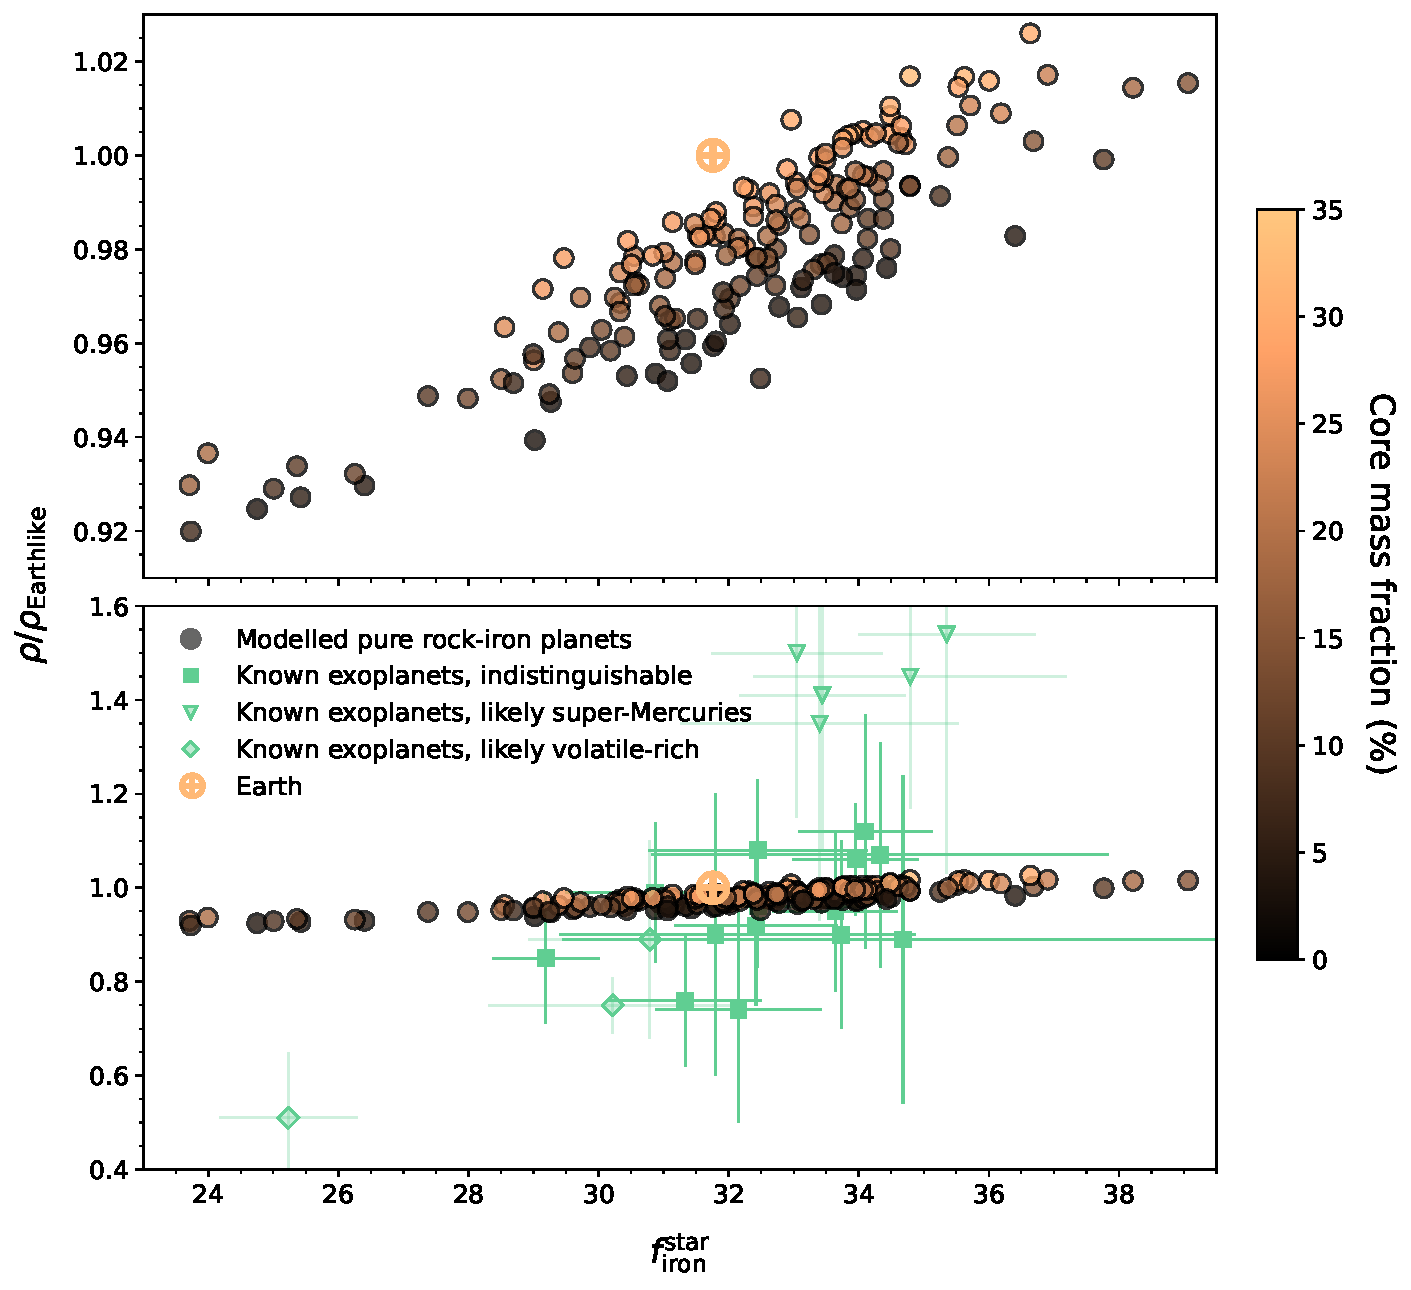
\includegraphics[width=\linewidth]{starplanet_stoich_subplot}
\caption[Test of the link between a planet's bulk density and host star iron abundance, quantifying the intrinsic bulk density scatter due to geochemistry.]{Test of the link between a planet's bulk density and host star iron abundance, quantifying the intrinsic bulk density scatter due to geochemistry \citep[cf.][Fig. 2]{adibekyan_compositional_2021}. The $y$-axis quantity $\rho / \rho_{\rm Earthlike}$ is the bulk density of the planet, scaled to the bulk density of a planet compositionally-identical to Earth. The $x$-axis quantity $f_{\rm iron}^{\rm star}$ is the wt.\% abundance of Fe in the bulk planet calculated from the host star abundances only, using the same stoichiometric method as \citet{adibekyan_compositional_2021} for consistency. Circles show the estimated bulk densities of synthetic Earth-mass planets ($N = 200$) with bulk compositions constrained by observed stellar refractory element abundances for a random sample of planet-hosting stars in the Hypatia Catalog. The synthetic planets have self-consistent mineralogy and density profiles, but ignore that iron cores could have liquid outer layers and/or contain light elements, which would change bulk densities by a few percent (a full description of the interior model is found in Chapter \ref{chapter:rockywater}). Earth's true bulk density is marked with a $\oplus$ symbol. For each modelled planet, the molar fraction of the total iron in its metal core is drawn from a random uniform prior distribition, $\mathcal{U}(0, 1)$, representing hard upper and lower intrinsic geochemical limits to core mass fraction, but not accounting for exogenous processes during planetary formation (e.g., collisional stripping of the mantle, which may have produced Mercury's core mass fraction of 0.7). The modelled core mass fractions (shown by the colourbar), and the modulations of $\rho / \rho_{\rm Earthlike}$ that result, are thus a function of the random Fe partitioning and the constrained stellar iron content. Green markers show the observed exoplanets from \citet{adibekyan_compositional_2021} sample, with triangles denoting the planets they identify as ``super-Mercuries'' (i.e., super-stellar iron core size), and the diamonds denoting the planets from this sample which \citet{unterborn_nominal_2023} identify as likely volatile-rich. The apparent positive correlation between $\rho / \rho_{\rm Earthlike}$ and $f_{\rm iron}^{\rm star}$ has been previously presented as evidence for a compositional link between planets and host stars in \citet{adibekyan_compositional_2021}. From the comparatively shallow slope of this correlation for the hypothetical pure rock-iron planets, after considering possible intrinsic variations in the extent of core formation, it appears that any perceived steeper slope cannot be explained by variations in stellar refractory abundances themselves.}
\label{fig:compositional-link} 
\end{figure}
%\todo{[TODO: show updated TOI-561 b density? scale to solar instead of observed Earth-density, needs recalculating scaled densities for the exoplanets. x-axis uncertainty?]}
% change f_iron_star method, show updated TOI-561 b density, maybe re-calculate scaled density with ExoPlex (better)?
% maybe scale to solar instead of observed Earth-density, needs recalculating scaled density




Figure \ref{fig:compositional-link} shows the exoplanet sample from \citet{adibekyan_compositional_2021}, on the same axes as their Fig. 2, but overlain by hypothetical pure metal-rock planets which I generated to have thermodynamically-consistent mineralogy based on observed stellar abundances \citep{hinkel_stellar_2014}, but with randomly assigned iron partitioning, $X_{\ce{Fe}}^{\rm metal}/(X_{\ce{Fe}}^{\rm metal} + X_{\ce{FeO}}^{\rm silicate})$, uniform between 0 and 1. It appears that the slope between the observed planet bulk density and the host star iron content is steeper than that which would be caused \textit{only} by stellar abudance variations with an unknown extent of core formation. Further, when compared to the synthetic planets, many of the exoplanets in this sample may be less dense than even a coreless planet, if their total iron content is otherwise constrained by the host star composition. These low densities would seem to require the presence of something else: high-molecular-mass atmospheres \citep{schulze_probability_2020}, deep water/steam layers \citep{kite_water_2021}, or magma oceans \citep{bower_linking_2019}. Therefore, the observed exoplanet bulk density variations would not be explained by stellar abundances alone. If the planet-star correlation, it is reported in \citet{adibekyan_compositional_2021}, is real, then we would need an explanation for why its slope is much greater than expected from mineralogy. If we cannot find such an explanation, then this particular correlation might be chance, or poor statistics. As such, it will be important to confirm how small planet volatile budgets relate to the iron abundance of their host star. %Whilst we might expect some sort of continuum of volatile layer thicknesses, very small mass fractions of water (much less than 1 wt.\%) can ensure a planet has no bare land surface, as I will show in Chapter \ref{chapter:topography}.

Nevertheless, \citet{schulze_probability_2020} and \citet{unterborn_nominal_2023} make the important point that the measurement uncertainty on both stellar abundance and planet bulk densities remains mostly too high to distinguish a volatile-enriched planet from an anemic one. High-precision observations of small planets around the most metal-poor, galactic thick-disc stars may be very useful to this end, statistically-speaking \citep[e.g.,][]{brinkman_toi561_2023}. An influence of orbital distances on planetary iron contents is also not strictly ruled out: \citet{mcdonough_terrestrial_2021} report an empirical correlation between the uncompressed densities of solar system bodies with their (current) heliocentric distance, and suggest this to be an effect of the Sun's magnetic field on these bodies' final Fe-metal contents. Whether the quoted effect is robust is not yet testable with observations of exoplanetary systems, however. It may be too early yet to attempt strong conclusions about a link between stellar iron content and planet composition, but we can anticipate improved measurement uncertainty and certainly a multiplying sample size in the near future.
% don't really trust adibekyan "f_iron^star" stoichiometry because it doesn't account for lower mantle being bridgmanite, kind of confusing, not sure if you should try to recreate it or just do in terms of refractory elements
% so far seems like oxidation state doesn't matter, scatter is negligible considering uncertainty, any trend therefore would to be volatiles / light element layers and can't be just from iron content
 
% not varying Si in core but mention how much bulk density difference this would make, also liquid outer core...
% verify with unterborn 2023 nominal range of bulk density - that paper agrees CMF does not have a large effect on bulk density even more so because liquid iron core is more compressible than the mantle. just looking at stellar iron content
% schulz paper's point is that measurement uncertainty too high to be certain that star inferred iron fraction is different than planet bulk density



%Notably, one planet in the \citet{adibekyan_compositional_2021} sample (TOI-561 b) has both anomalously low bulk density and low host-star Fe content---TOI-561 being a metal-poor star in the galactic thick disc. Adding more rocky planets around significantly metal-poor stars to this plot might reveal a clear association between extreme variations in stellar iron content and planet bulk density. However, as it stands, the data point from TOI-561 b would seem to carry disproportional weight in the linear regression, and it would be interesting to see if there is still a statistically significant correlation for thin disc stars only (which vary in Fe abundance by just a few percent). %From Schultze et al it might be pointed out that even if we can't reject the fact that planet core size is not directly related to star iron within the uncertainty, doesn't automatically mean they are predictable. 

%One point seem clear, which is that if we pretend planets are pure iron cores and pure \ce{MgSiO3} mantles, then the empirical core (= iron) mass fractions inferred from bulk density show a broader distribution than the emprical iron mass fractions implied by stellar Fe/(Mg + Si) \citep{plotnykov_chemical_2020}. Therefore, other processes are operating to set planets' core sizes, at the level of accretion, differentiation, or both. More precisely-measured planets in this size regime may give us a better idea of whether this star-planet correlation indeed exists and provides meaningful information on core sizes.





I think it is also worth revisiting here a study by \citet{doyle_oxygen_2019}, measuring FeO abundances in polluted white dwarfs, which is often cited as empirical evidence that most rocky planets have similar $X_{\ce{Fe}}^{\rm metal}/X_{\ce{FeO}}^{\rm silicate}$ to Earth (i.e., equilibrium \eqref{eq:background-iw} is at the same position). Yet insofar as the observed instantaneous pollutant composition does not represent an entire parent body \citep[e.g.,][]{brouwers_asynchronous_2022, brouwers_asynchronous_2023}, the parent body's total iron budget is unknown, and whilst we might be estimating $X_{\ce{FeO}}^{\rm silicate}$ we cannot constrain the iron partitioning from these observations alone. Hence \citet{doyle_oxygen_2019} must assume an Earth-like $X_{\ce{Fe}}^{\rm metal}$. This problem is in addition to the sometimes-unappreciated difficulty in accurately measuring O abundances in polluted white dwarfs (section \ref{sec:background-pwd}). 


To reiterate, the relative iron core sizes of planets are a crucial and poorly-constrained aspect of their characterisation and evolution. I have introduced three reasons why (but there are more). Firstly, because the core radius controls the mantle depth ($d$ in equation (\ref{eq:Ra-background})), it can be just as important as the planet radius in determining the vigour of convection---one of the key parameters governing planets' thermal histories---hence their volcanism, tectonics, and volatile cycling. Secondly, core Fe-metal trades off with mantle Fe oxide, such that for the same bulk Fe inventory, smaller cores imply more FeO in the mantle, which, on top of lowering its viscosity \citep{zhao_effect_2009}, also increases melt productivity \citep{hirschmann_mantle_2000, kiefer_effects_2015}, thickening the juvenile crust that forms from partial melting of this mantle \citep{wade_divergent_2017, dyck_effect_2021}---the consequentially greater volume of hydrous crustal minerals may have contributed to the loss of surface water on Mars \citep{wade_divergent_2017}. Thirdly, estimating the the likelihood of an observed planet being rocky, based on its bulk density and host star abundances, requires an informative prior distribution of core mass fraction. %Although a slighly larger or smaller core may not affect a planet's observed density, it will certainly affect its overall evolution.
This thesis does not aim to make progress towards constraining rocky planet core sizes; nevertheless, it is important to introduce as a limiting problem shared by many exoplanet scientists, from the Earth-up to the space-down. 





%\todo{theory directions: core/silicate mass ratio is set by redox conditions during core formation through equilibria, and a priori we can't say if we expect these to be broadly similar across most rocky planets, therefore CMF not predictable from first principles. Further, core size directly relates to thermal history through affecting the mantle depth, thus having a similar direct consequence as planet mass (eq. Ra); it also relates to mantle iron oxide content which can have far-reaching implications e.g. the the thickness and density of a crust that forms (wade, dyck).}




\section{A big weird universe}

%\todo{e.g, tidal locking, stellar energy distributions, orbital configurations (ellipticity)...Impossible to cover all of these in a study or six... we mention these to avoid upsetting anyone who has a favourite piece of planetary diversity that they have dedicated themselves to the research of, because probably all of this is equally important.---note these things are not internal planet effects so maybe don't even need to mention} 

%Intelligent life capable of observing the solar system would probably think that our terrestrial planets are just as strange.

Despite this thesis' narrative of general trends in prototypical planets, the universe does not make astronomical objects that are all identical save some parameter. Real planets have idiosyncracy. Many of the known rocky worlds, so far the easiest for us to detect, orbit so close to their stars as to be tidally-locked: with a permanent day side and night side, like the Moon is to Earth. Simulations of mantle convection on tidally-locked planets have shown the extreme hemispheric contrast in surface temperature could influence their mantle convection \citep{vansummeren_mantle_2011, gelman_effects_2011, meier_hemispheric_2021}---in stark contrast to the planets discussed here, where stellar radiation has no effect on interior evolution. Some of these worlds, like CoRoT-7 b and 55 Cancri e, are kept so exceedingly hot that they may remain molten for billions of years, never crystallising a mantle \citep{leger_transiting_2009, demory_map_2016}. Other internal heating mechanisms could operate on short-period exoplanets, namely tidal dissipation \citep{driscoll_tidal_2015, renaud_increased_2018, dobos_tidal_2019} and induction heating by the stellar magnetic field \citep{kislyakova_electromagnetic_2020, grayver_interior_2022}. Of course interior convection is just as holistically important on these planets, but it will be in a different regime; ``generalised" thermal evolutions cannot be extrapolated across different regimes of convection, as I have stressed. Magnetic fields and their consequences are not addressed here, although they are a direct outcome of thermal evolution and so convection models have been used to predict their likelihoods \citep{nimmo_why_2002, gaidos_thermodynamic_2010, driscoll_thermal_2014, Foley2016, boujibar_superearth_2020, zhang_thermal_2022}. Also influencing a planet's surface, of course, are the astrophysical factors: non-circular orbits \citep{williams_earthlike_2002, dobrovolskis_spin_2007, way_effects_2017, palubski_habitability_2020}, for example, or the spectral energy distribution of the host star \citep{kasting_ultraviolet_1997, shields_effect_2013, godolt_3d_2015, eager-nash_implications_2020}, all getting their dedicated attention elsewhere. It is impossible to %cover everyone's favourite aspect of exoplanet diversity, 
cover every factor causing rocky planets to diverge, but this chapter has covered what I believe to be the most salient ones.
% Throughout this section I have explained the assumptions and simplifications that make planetary interior models tractable.

% moons, but moonless earth probably not uninhabitable latest simulations

% .magnetic fields seem relevant for UV shielding and atmospheric stripping \citep{dong_atmospheric_2020}, but is clearly not the only thing comparing Venus to Earth , and may not be a sufficient condition \citep{gunell_why_2018}




\section{Structure of the thesis}



This thesis combines foundational planetary science, state-of-the-art numerical tools, and nimble box-model insights to investigate several cases of rocky planet diversity from the inside out. In doing so, I make some contribution towards several core research questions:

\begin{itemize}

\item How easily is surface topography generated on planets?
\item To what extent do stagnant lid planets cycle their volatiles between interior and surface?
\item Does stellar chemistry influence the volatile composition of planetary mantles, their magmas, and their derived volcanic gases?

\end{itemize}


\textbf{Chapter \ref{chapter:topography}} estimates the heights of intrinsic topography on rocky planets which is a basic consequence of their mantle convection. Topography carves out basins to contain surface water, so planets with higher topography would be more prone to having islands above sea level. \textbf{Chapter \ref{chapter:outgassing}} then applies a mantle convection model to pre-plate tectonics Archean Earth, questioning the contemporaneous high rates of volcanic outgassing inferred when classic thermal history models \citep[e.g.,][]{schubert_whole_1980} are extrapolated backwards in time. Archean Earth presents a useful case study to explore in-depth with justifiably more-sophisticated numerical models. %, such as the one here coupling convection with melting and redox chemistry. 
\textbf{Chapter \ref{chapter:rockywater}}, recognising that exoplanets' initial interior water contents have never been constrained---but are a principle factor affecting water outgassing rates (from Chapter \ref{chapter:outgassing})---predicts the maximum water that would be stored in mantle minerals across the expected range of bulk compositions. Lastly, in \textbf{Chapter \ref{chapter:fo2}}, I show that there must be at least a multiple-order-of-magnitude variation in how oxidising these mantles will be across the same range in bulk composition. Given that small changes in redox conditions can have large consequences for petrological and atmospheric evolution on planets, these last results emphasise even more how modern Earth represents a specific outcome of thermal-chemical-geodynamic evolution; planet Earth is fading as the old cosmic modality. \textbf{Chapter \ref{chapter:conclusion}} synthesises this work under the loose theme of water and life on rocky worlds. 

